\chapter{Experiments}
\label{chapter:experiments}

%\subcaptionbox{Training Curve-Fitting}{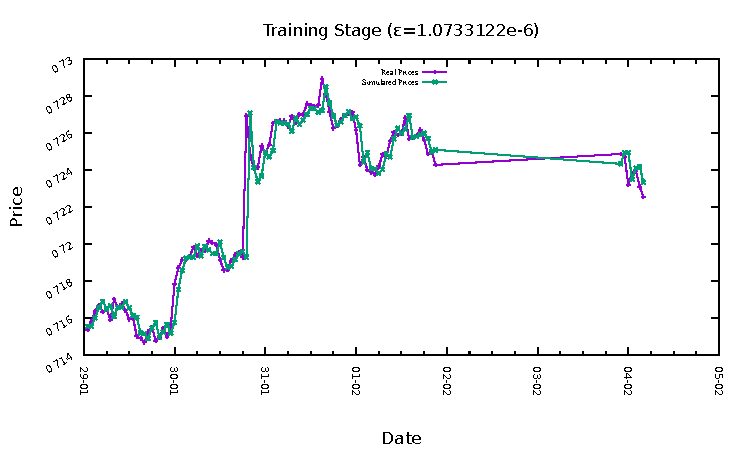
\includegraphics[width=.45\textwidth]{img/plots/aud_usd_h1-10agents-10rules-20ind-100gen_training_fit.pdf}}\quad
%subcaptionbox{}{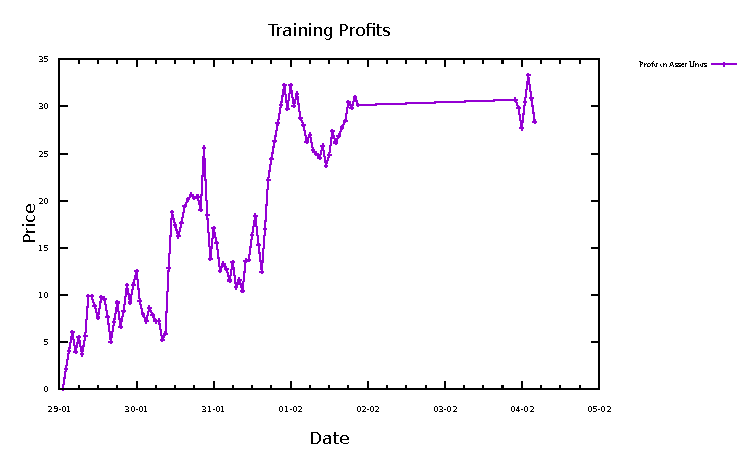
\includegraphics[width=.45\textwidth]{img/plots/aud_usd_h1-10agents-10rules-20ind-100gen_training_profits.pdf}}

This Chapter describes a series of experiments that were performed in order to
demonstrate the capabilities of the proposed method regarding two areas:
forecasting and interpretability. The forecasting capabilities of the method are
demonstrated by exhibiting how the multi-agent model simulates the prices in
training and testing datasets, and how the system's curve-fitting error
decreased throughout the genetic algorithm's generations. The simulated profits
are also included, for both the training and testing datasets. Regarding the
interpretation capabilities of the method, a description of how the agents
perceive the market is shown. This description also describes what actions the
agents take according to their perceptions.

A total of 135 experiments were performed, but due to space constraints in this
thesis document, only some of the experiments are shown. The reader can find the
plots and interpretations for all the experiments performed in the Git
repository of this thesis here: https://github.com/amherag/PhD-Thesis/.

% All 100 gen, same range of time
% We sort by number of agents and then by profit in insights

\section{Forecasting the Prices of a Financial Market}
\label{section:forecasting-the-prices-of-a-financial-market}

\subsection{AUD/USD 4 Agents, 4 Rules, 4 Individuals}
\label{results:forecast-aud-usd-4agents-4rules-4individuals}

\begin{figure}[htp]
  \centering

  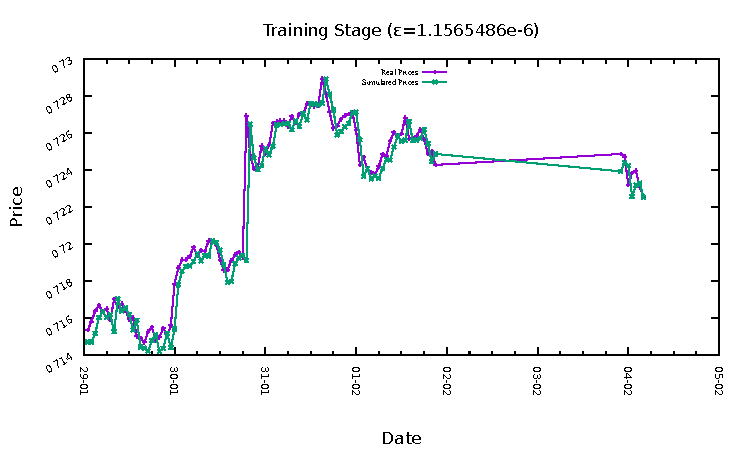
\includegraphics[width=.45\textwidth]{img/plots/aud_usd_h1-4agents-4rules-4ind-100gen_training_fit.pdf}\quad
  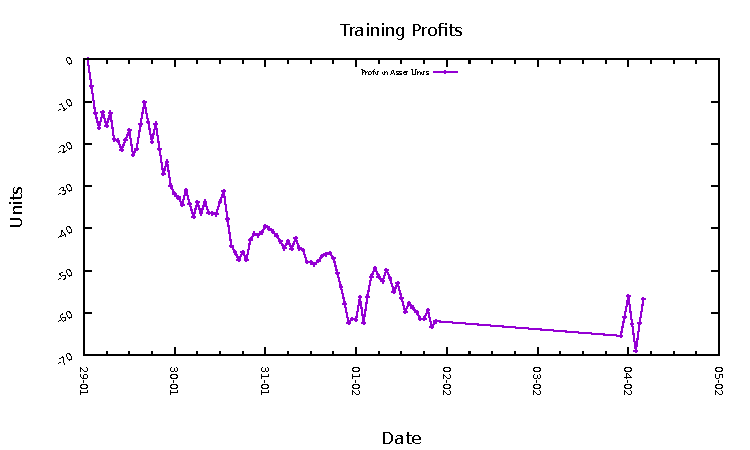
\includegraphics[width=.45\textwidth]{img/plots/aud_usd_h1-4agents-4rules-4ind-100gen_training_profits.pdf}

  \medskip

  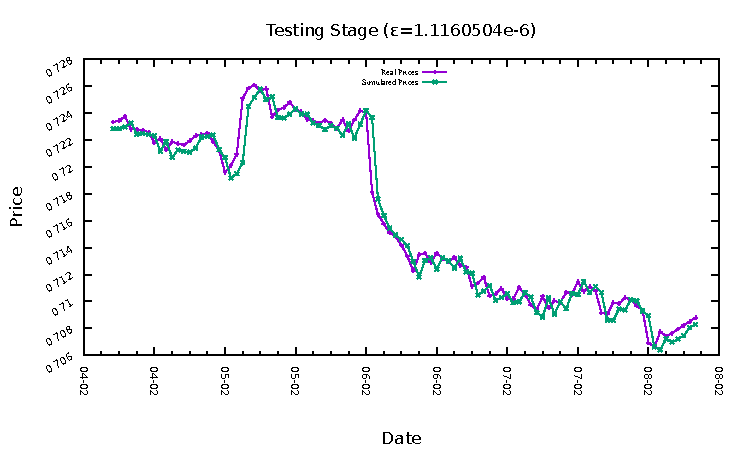
\includegraphics[width=.45\textwidth]{img/plots/aud_usd_h1-4agents-4rules-4ind-100gen_testing_fit.pdf}\quad
  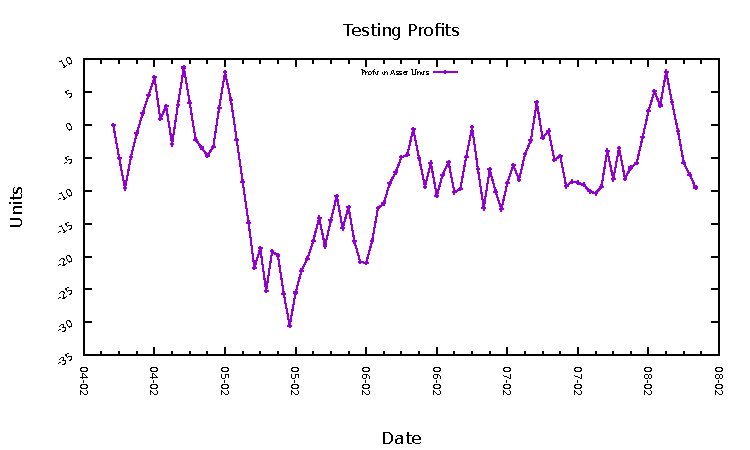
\includegraphics[width=.45\textwidth]{img/plots/aud_usd_h1-4agents-4rules-4ind-100gen_testing_profits.pdf}

  \medskip

  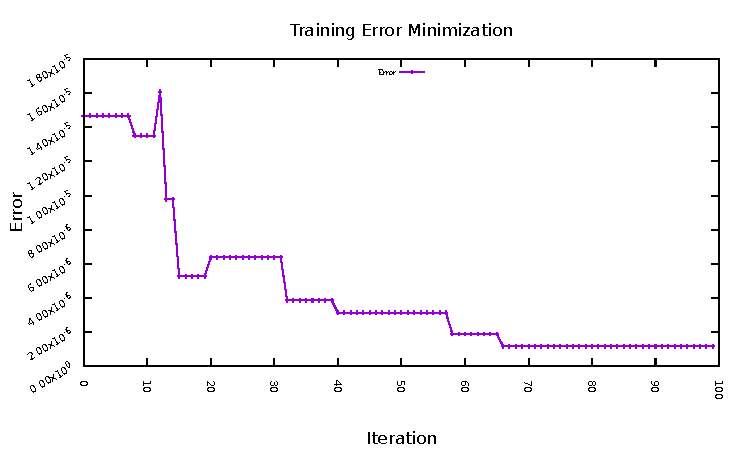
\includegraphics[width=.45\textwidth]{img/plots/aud_usd_h1-4agents-4rules-4ind-100gen_error_minimization.pdf}

  \caption{AUD/USD - 4 agents, 4 rules and 4 individuals}
  \label{pics:aud-usd-4agents-4rules-4individuals}
\end{figure}

\subsection{AUD/USD 10 Agents, 10 Rules, 10 Individuals}
\label{results:forecast-aud-usd-10agents-10rules-10individuals}

\begin{figure}[htp]
  \centering

  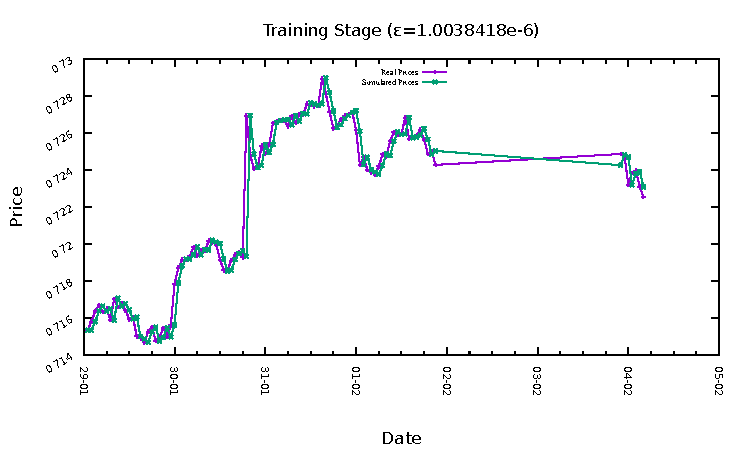
\includegraphics[width=.45\textwidth]{img/plots/aud_usd_h1-10agents-10rules-10ind-100gen_training_fit.pdf}\quad
  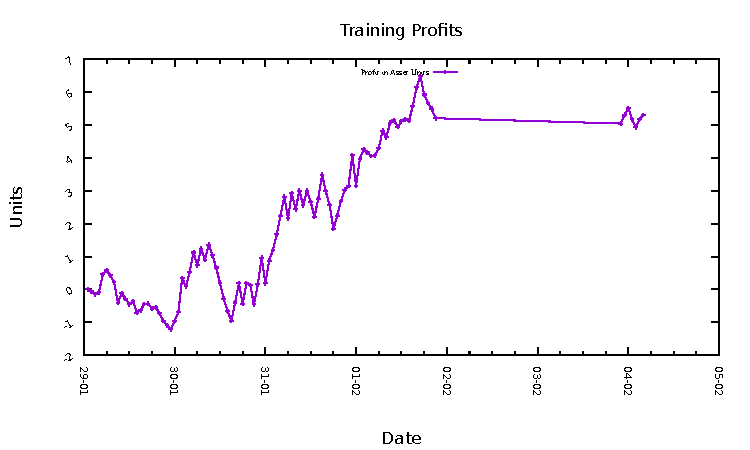
\includegraphics[width=.45\textwidth]{img/plots/aud_usd_h1-10agents-10rules-10ind-100gen_training_profits.pdf}

  \medskip

  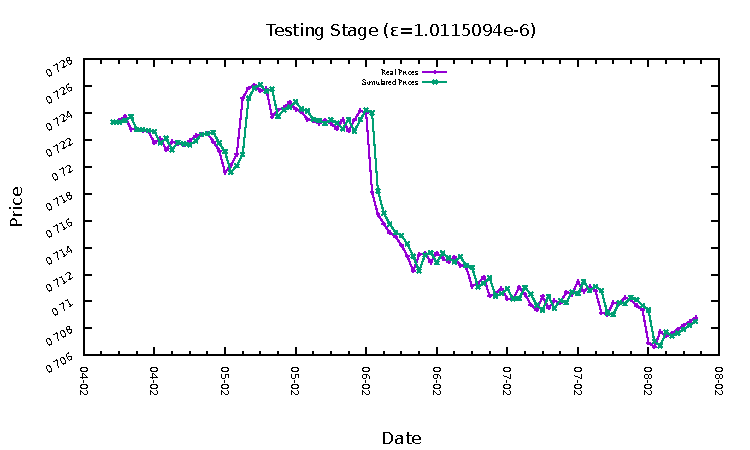
\includegraphics[width=.45\textwidth]{img/plots/aud_usd_h1-10agents-10rules-10ind-100gen_testing_fit.pdf}\quad
  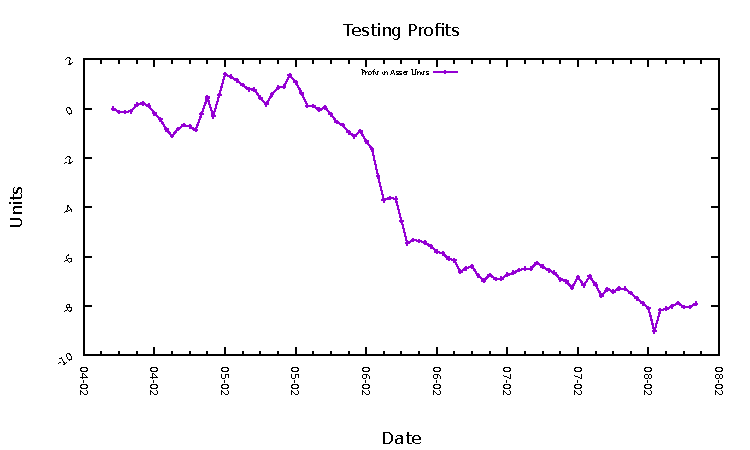
\includegraphics[width=.45\textwidth]{img/plots/aud_usd_h1-10agents-10rules-10ind-100gen_testing_profits.pdf}

  \medskip

  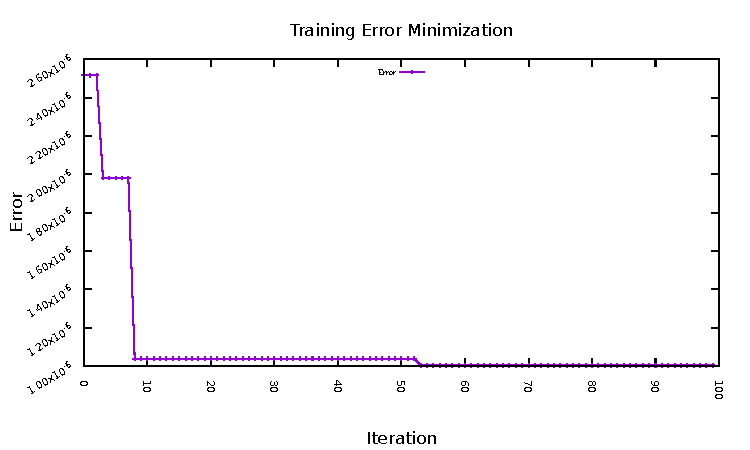
\includegraphics[width=.45\textwidth]{img/plots/aud_usd_h1-10agents-10rules-10ind-100gen_error_minimization.pdf}

  \caption{AUD/USD - 10 agents, 10 rules and 10 individuals}
  \label{pics:aud-usd-10agents-10rules-10individuals}
\end{figure}

\subsection{AUD/USD 20 Agents, 20 Rules, 20 Individuals}
\label{results:forecast-aud-usd-20agents-20rules-20individuals}

\begin{figure}[htp]
  \centering

  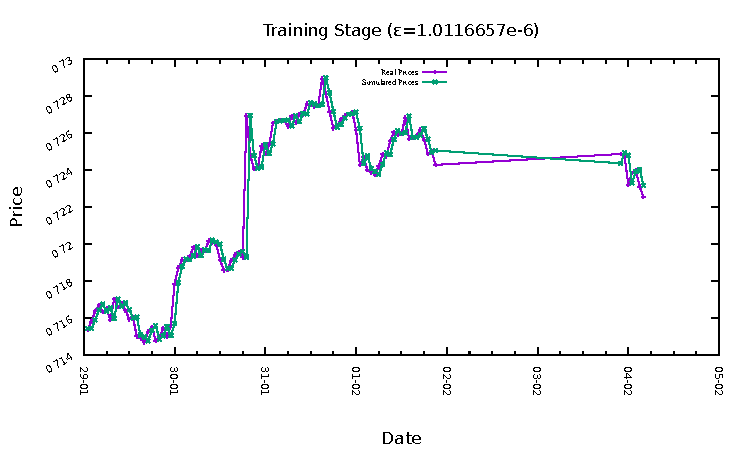
\includegraphics[width=.45\textwidth]{img/plots/aud_usd_h1-20agents-20rules-20ind-100gen_training_fit.pdf}\quad
  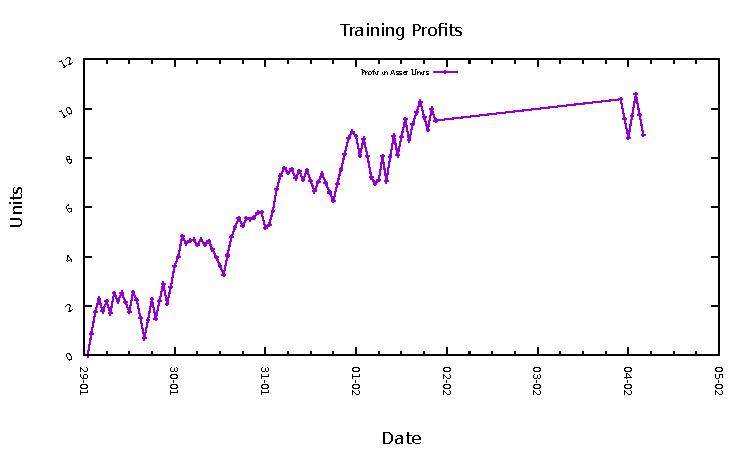
\includegraphics[width=.45\textwidth]{img/plots/aud_usd_h1-20agents-20rules-20ind-100gen_training_profits.pdf}

  \medskip

  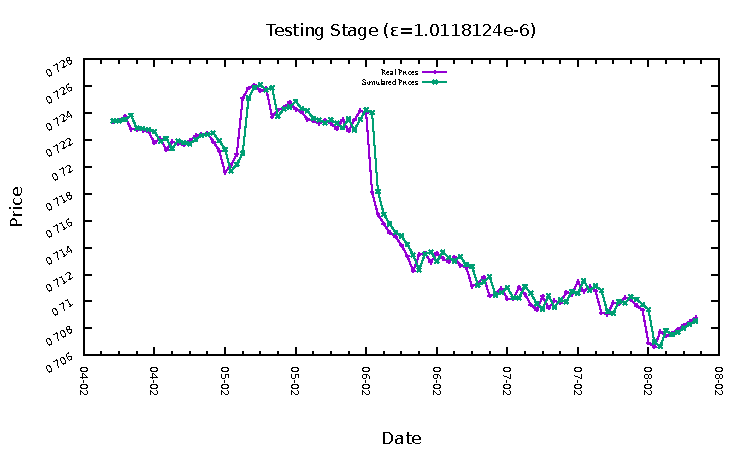
\includegraphics[width=.45\textwidth]{img/plots/aud_usd_h1-20agents-20rules-20ind-100gen_testing_fit.pdf}\quad
  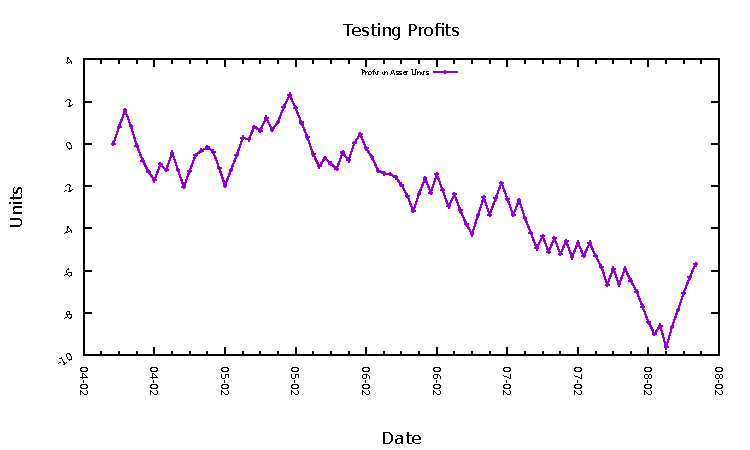
\includegraphics[width=.45\textwidth]{img/plots/aud_usd_h1-20agents-20rules-20ind-100gen_testing_profits.pdf}

  \medskip

  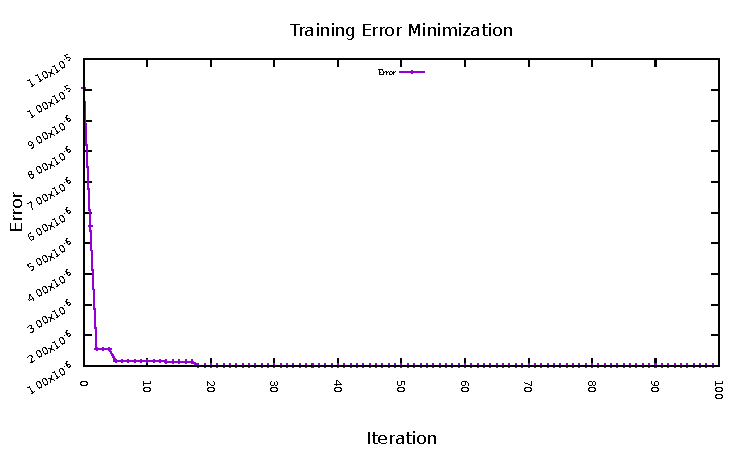
\includegraphics[width=.45\textwidth]{img/plots/aud_usd_h1-20agents-20rules-20ind-100gen_error_minimization.pdf}

  \caption{AUD/USD - 20 agents, 20 rules and 20 individuals}
  \label{pics:aud-usd-20agents-20rules-20individuals}
\end{figure}








\subsection{EUR/GBP 4 Agents, 4 Rules, 4 Individuals}
\label{results:forecast-eur-gbp-4agents-4rules-4individuals}

\begin{figure}[htp]
  \centering

  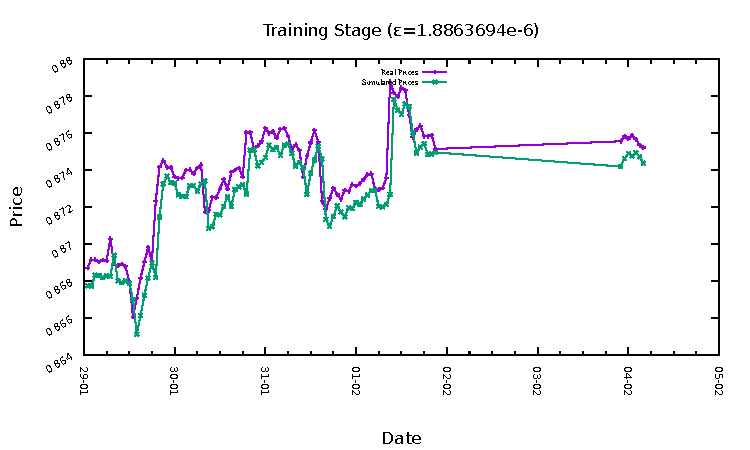
\includegraphics[width=.45\textwidth]{img/plots/eur_gbp_h1-4agents-4rules-4ind-100gen_training_fit.pdf}\quad
  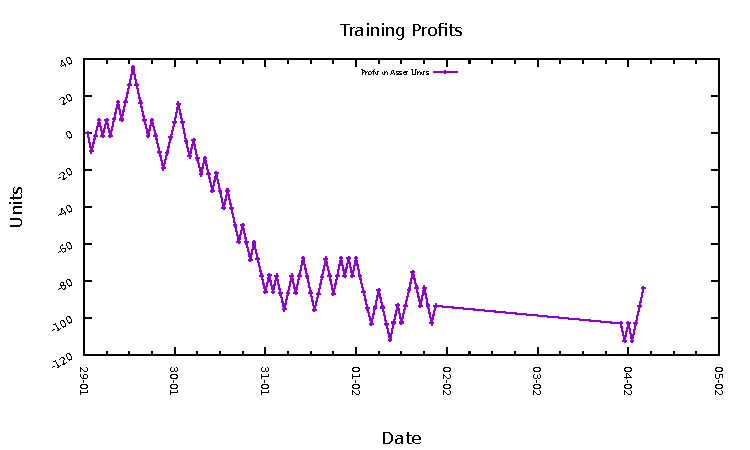
\includegraphics[width=.45\textwidth]{img/plots/eur_gbp_h1-4agents-4rules-4ind-100gen_training_profits.pdf}

  \medskip

  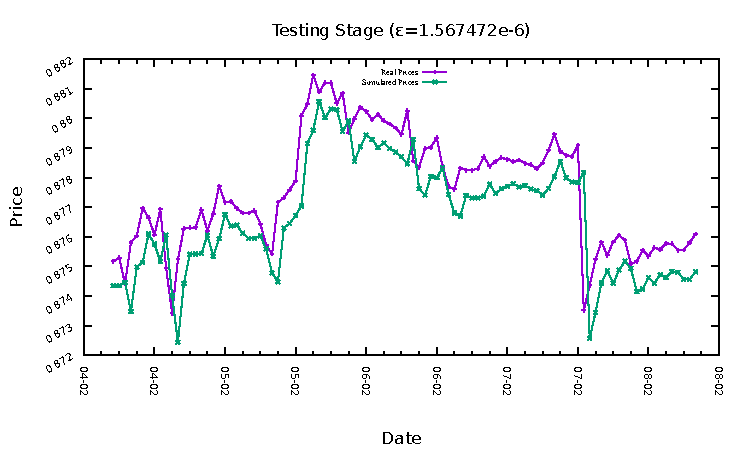
\includegraphics[width=.45\textwidth]{img/plots/eur_gbp_h1-4agents-4rules-4ind-100gen_testing_fit.pdf}\quad
  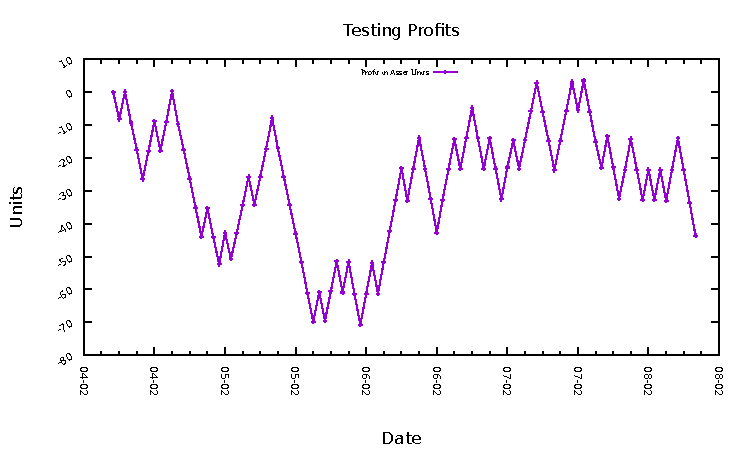
\includegraphics[width=.45\textwidth]{img/plots/eur_gbp_h1-4agents-4rules-4ind-100gen_testing_profits.pdf}

  \medskip

  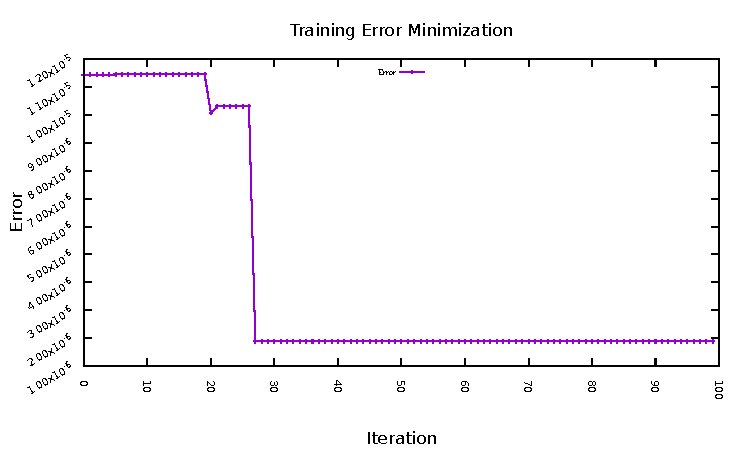
\includegraphics[width=.45\textwidth]{img/plots/eur_gbp_h1-4agents-4rules-4ind-100gen_error_minimization.pdf}

  \caption{EUR/GBP - 4 agents, 4 rules and 4 individuals}
  \label{pics:eur-gbp-4agents-4rules-4individuals}
\end{figure}

\subsection{EUR/GBP 10 Agents, 10 Rules, 10 Individuals}
\label{results:forecast-eur-gbp-10agents-10rules-10individuals}

\begin{figure}[htp]
  \centering

  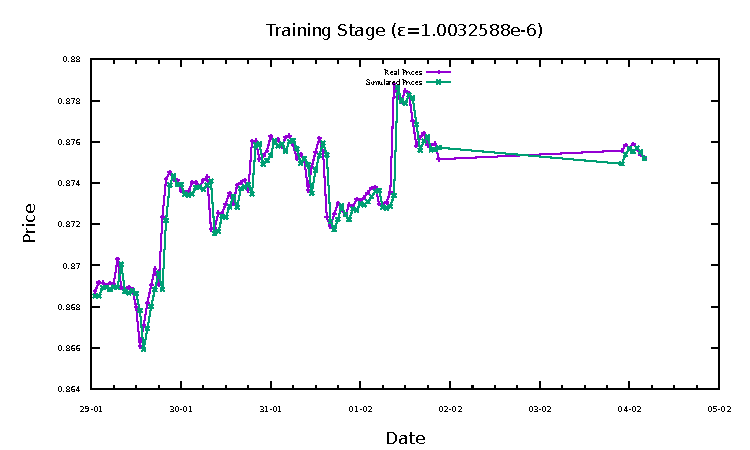
\includegraphics[width=.45\textwidth]{img/plots/eur_gbp_h1-10agents-10rules-10ind-100gen_training_fit.pdf}\quad
  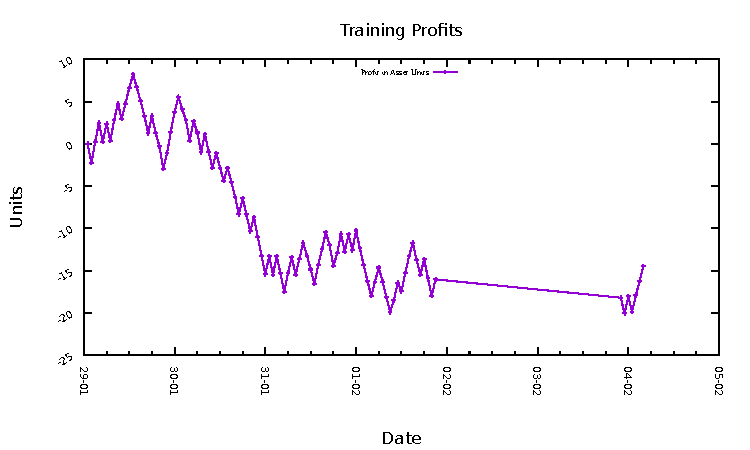
\includegraphics[width=.45\textwidth]{img/plots/eur_gbp_h1-10agents-10rules-10ind-100gen_training_profits.pdf}

  \medskip

  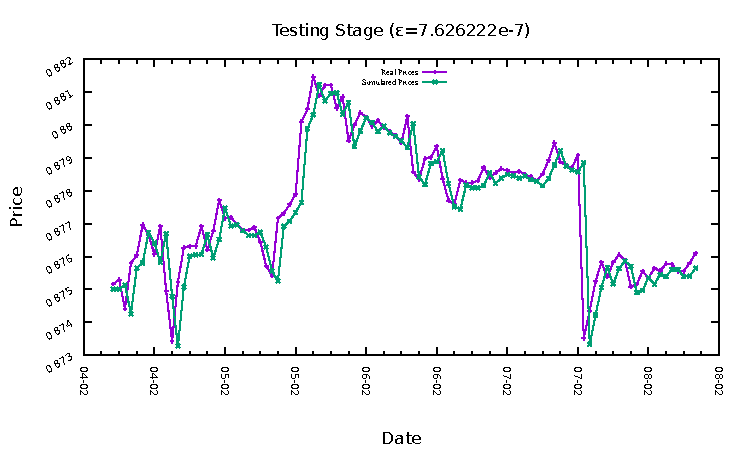
\includegraphics[width=.45\textwidth]{img/plots/eur_gbp_h1-10agents-10rules-10ind-100gen_testing_fit.pdf}\quad
  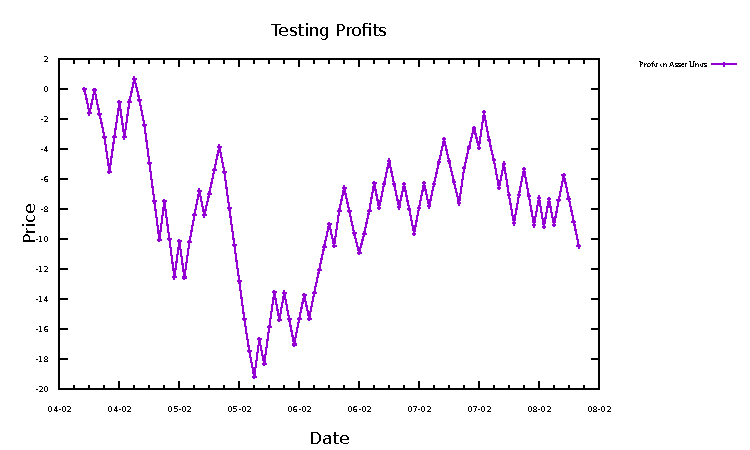
\includegraphics[width=.45\textwidth]{img/plots/eur_gbp_h1-10agents-10rules-10ind-100gen_testing_profits.pdf}

  \medskip

  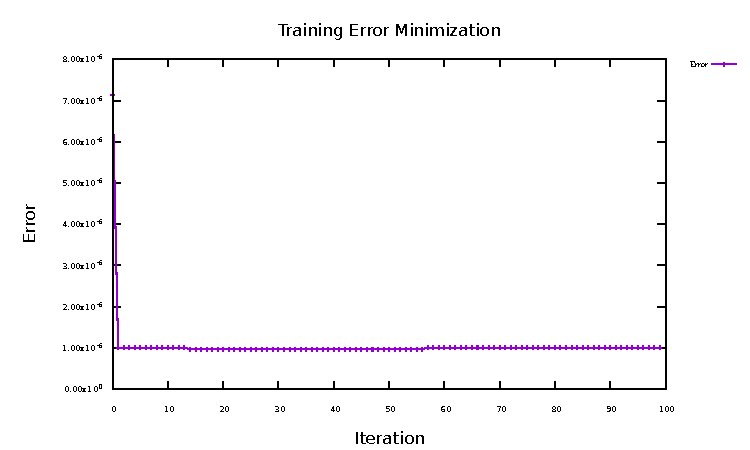
\includegraphics[width=.45\textwidth]{img/plots/eur_gbp_h1-10agents-10rules-10ind-100gen_error_minimization.pdf}

  \caption{EUR/GBP - 10 agents, 10 rules and 10 individuals}
  \label{pics:eur-gbp-10agents-10rules-10individuals}
\end{figure}

\subsection{EUR/GBP 20 Agents, 20 Rules, 20 Individuals}
\label{results:forecast-eur-gbp-20agents-20rules-20individuals}

\begin{figure}[htp]
  \centering

  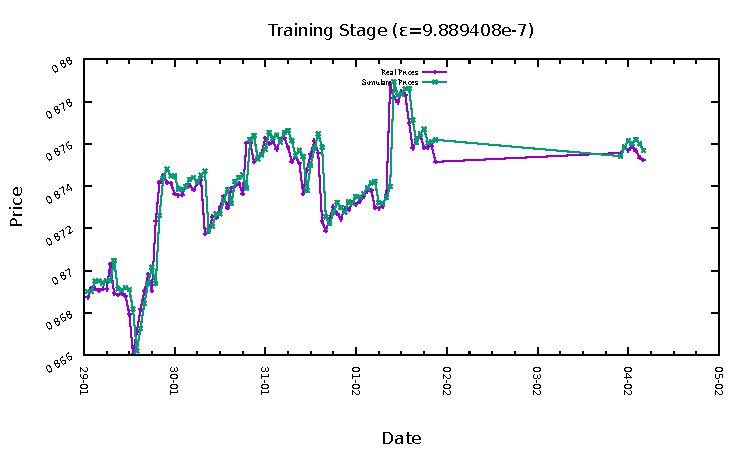
\includegraphics[width=.45\textwidth]{img/plots/eur_gbp_h1-20agents-20rules-20ind-100gen_training_fit.pdf}\quad
  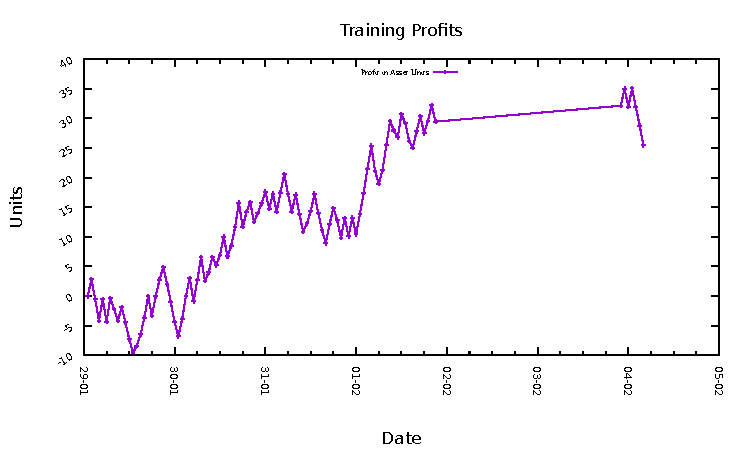
\includegraphics[width=.45\textwidth]{img/plots/eur_gbp_h1-20agents-20rules-20ind-100gen_training_profits.pdf}

  \medskip

  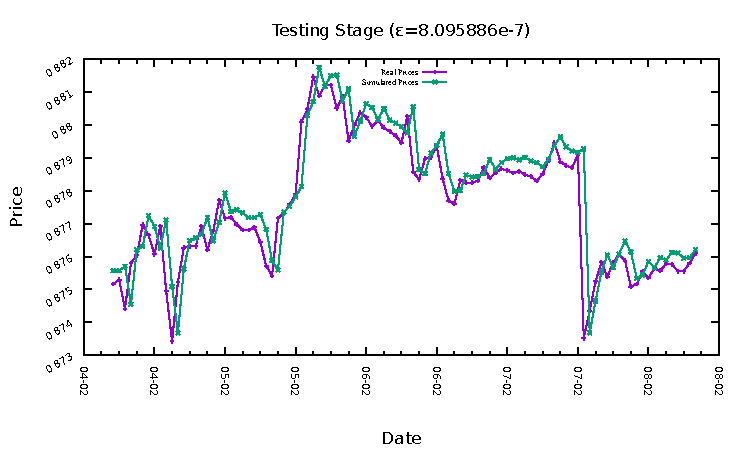
\includegraphics[width=.45\textwidth]{img/plots/eur_gbp_h1-20agents-20rules-20ind-100gen_testing_fit.pdf}\quad
  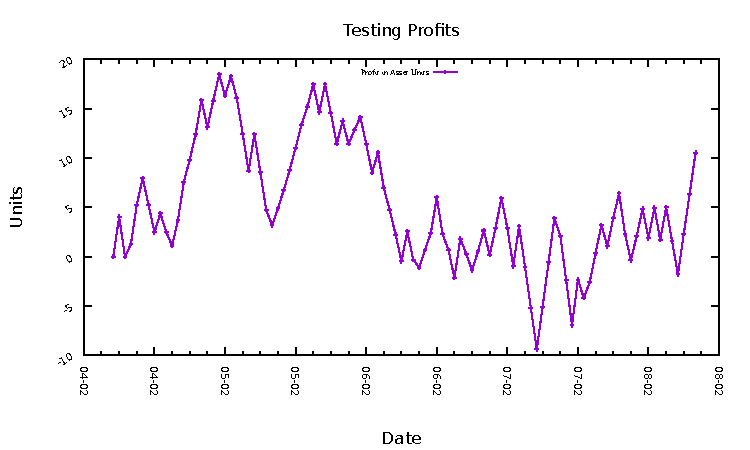
\includegraphics[width=.45\textwidth]{img/plots/eur_gbp_h1-20agents-20rules-20ind-100gen_testing_profits.pdf}

  \medskip

  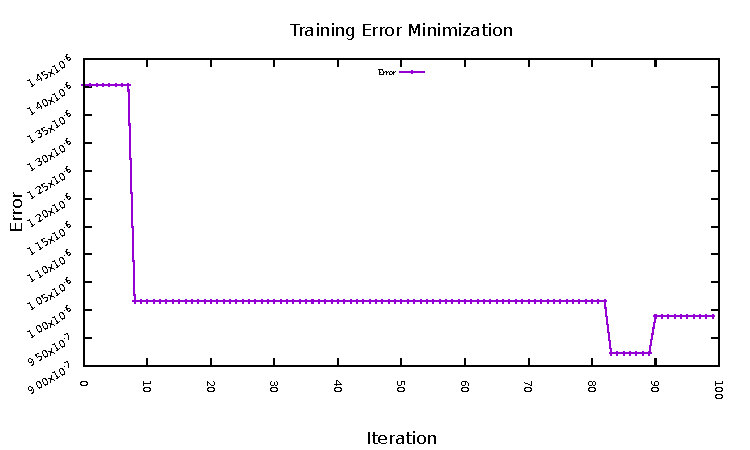
\includegraphics[width=.45\textwidth]{img/plots/eur_gbp_h1-20agents-20rules-20ind-100gen_error_minimization.pdf}

  \caption{EUR/GBP - 20 agents, 20 rules and 20 individuals}
  \label{pics:eur-gbp-20agents-20rules-20individuals}
\end{figure}






\subsection{EUR/USD 4 Agents, 4 Rules, 4 Individuals}
\label{results:forecast-eur-usd-4agents-4rules-4individuals}

\begin{figure}[htp]
  \centering

  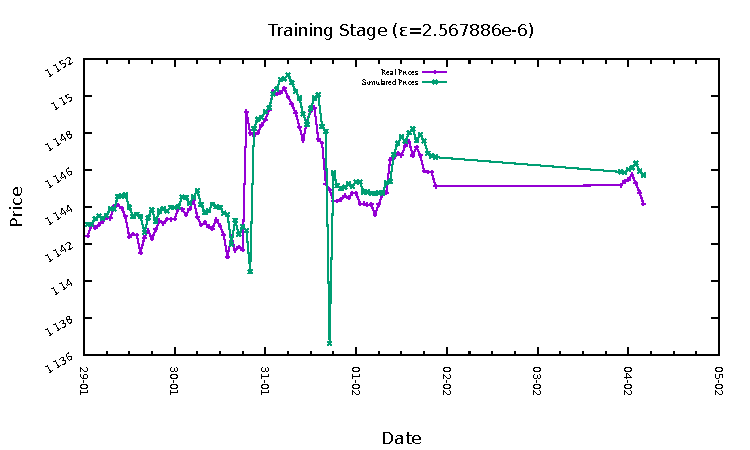
\includegraphics[width=.45\textwidth]{img/plots/eur_usd_h1-4agents-4rules-4ind-100gen_training_fit.pdf}\quad
  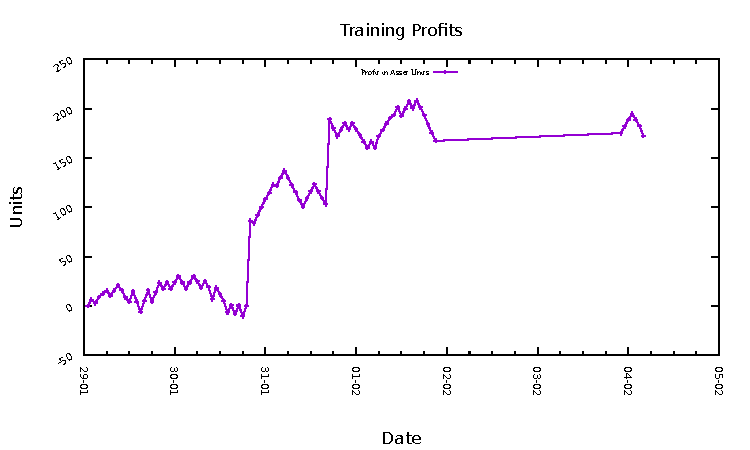
\includegraphics[width=.45\textwidth]{img/plots/eur_usd_h1-4agents-4rules-4ind-100gen_training_profits.pdf}

  \medskip

  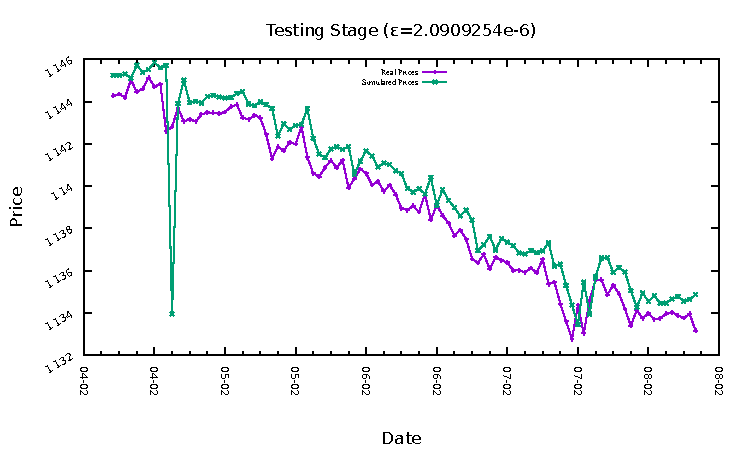
\includegraphics[width=.45\textwidth]{img/plots/eur_usd_h1-4agents-4rules-4ind-100gen_testing_fit.pdf}\quad
  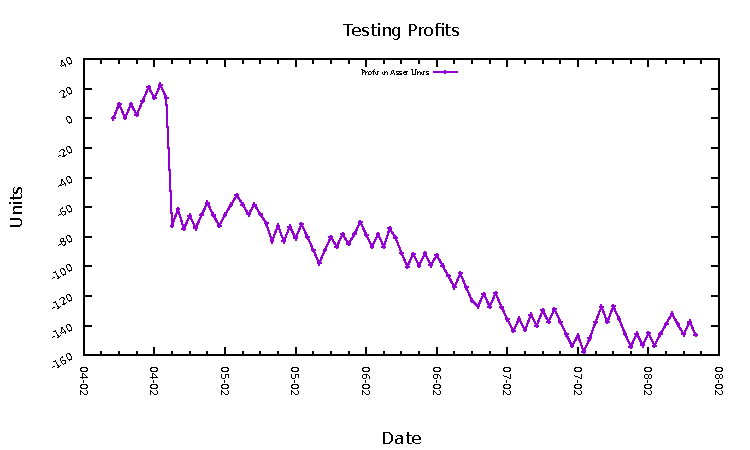
\includegraphics[width=.45\textwidth]{img/plots/eur_usd_h1-4agents-4rules-4ind-100gen_testing_profits.pdf}

  \medskip

  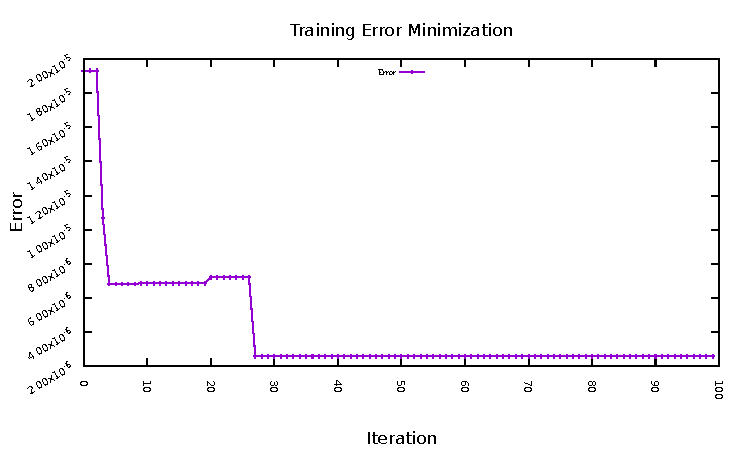
\includegraphics[width=.45\textwidth]{img/plots/eur_usd_h1-4agents-4rules-4ind-100gen_error_minimization.pdf}

  \caption{EUR/USD - 4 agents, 4 rules and 4 individuals}
  \label{pics:eur-usd-4agents-4rules-4individuals}
\end{figure}

\subsection{EUR/USD 10 Agents, 10 Rules, 10 Individuals}
\label{results:forecast-eur-usd-10agents-10rules-10individuals}

\begin{figure}[htp]
  \centering

  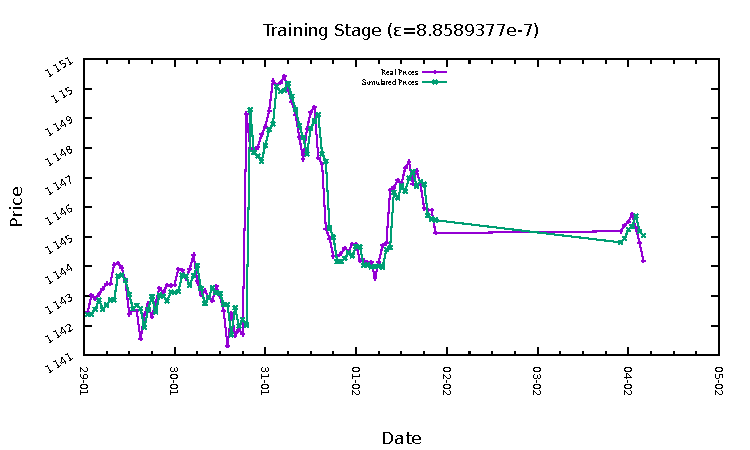
\includegraphics[width=.45\textwidth]{img/plots/eur_usd_h1-10agents-10rules-10ind-100gen_training_fit.pdf}\quad
  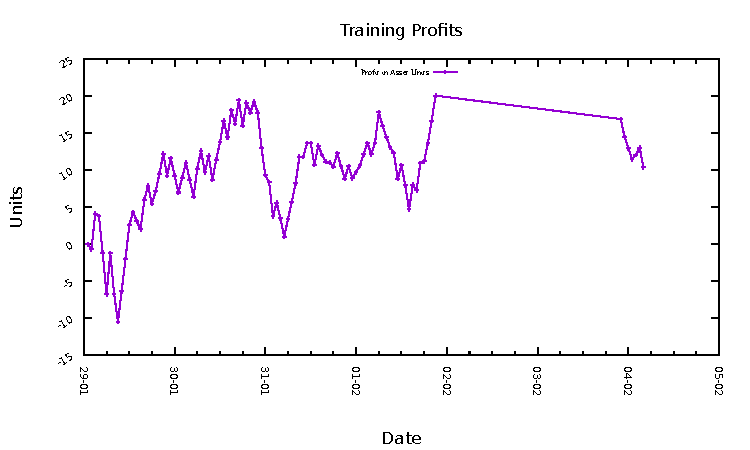
\includegraphics[width=.45\textwidth]{img/plots/eur_usd_h1-10agents-10rules-10ind-100gen_training_profits.pdf}

  \medskip

  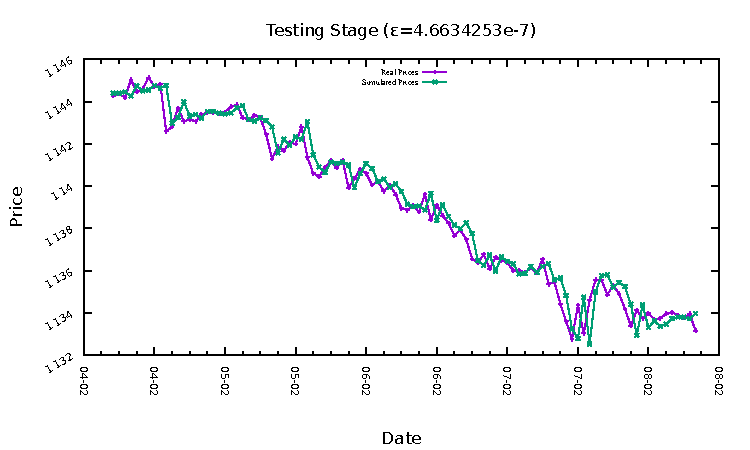
\includegraphics[width=.45\textwidth]{img/plots/eur_usd_h1-10agents-10rules-10ind-100gen_testing_fit.pdf}\quad
  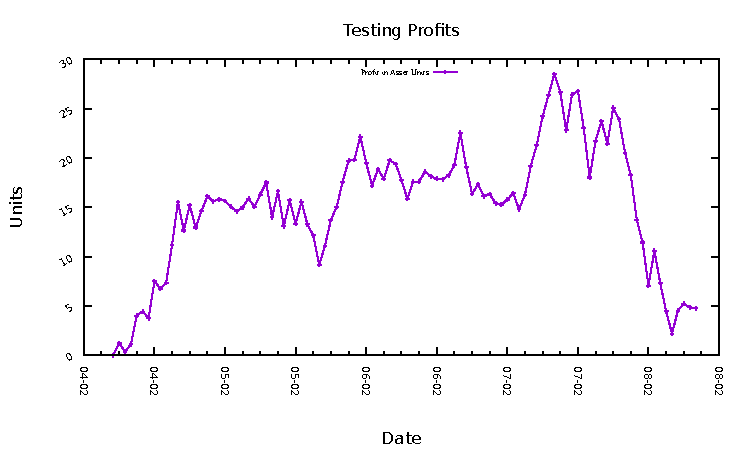
\includegraphics[width=.45\textwidth]{img/plots/eur_usd_h1-10agents-10rules-10ind-100gen_testing_profits.pdf}

  \medskip

  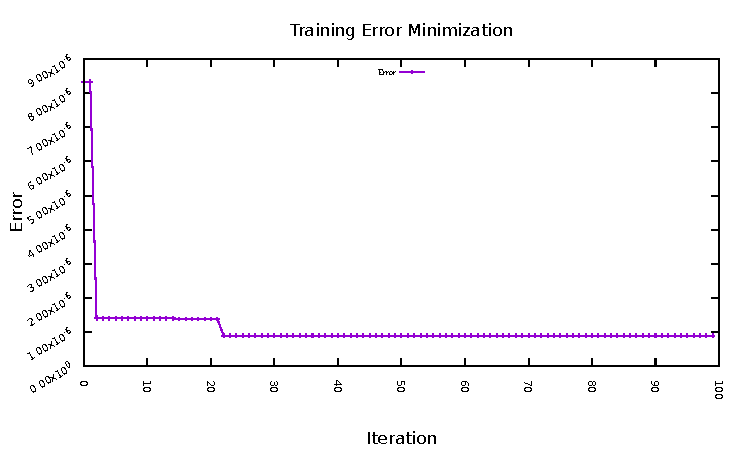
\includegraphics[width=.45\textwidth]{img/plots/eur_usd_h1-10agents-10rules-10ind-100gen_error_minimization.pdf}

  \caption{EUR/USD - 10 agents, 10 rules and 10 individuals}
  \label{pics:eur-usd-10agents-10rules-10individuals}
\end{figure}

\subsection{EUR/USD 20 Agents, 20 Rules, 20 Individuals}
\label{results:forecast-eur-usd-20agents-20rules-20individuals}

\begin{figure}[htp]
  \centering

  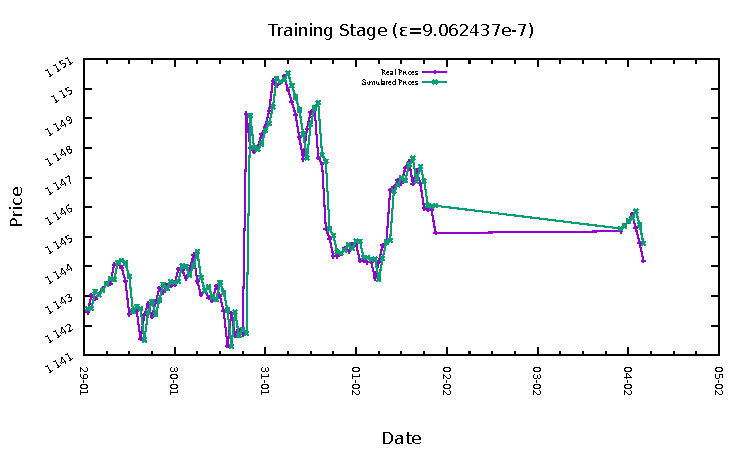
\includegraphics[width=.45\textwidth]{img/plots/eur_usd_h1-20agents-20rules-20ind-100gen_training_fit.pdf}\quad
  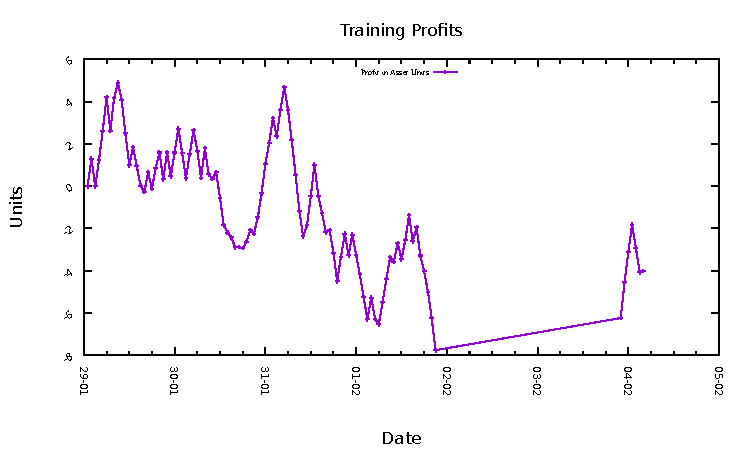
\includegraphics[width=.45\textwidth]{img/plots/eur_usd_h1-20agents-20rules-20ind-100gen_training_profits.pdf}

  \medskip

  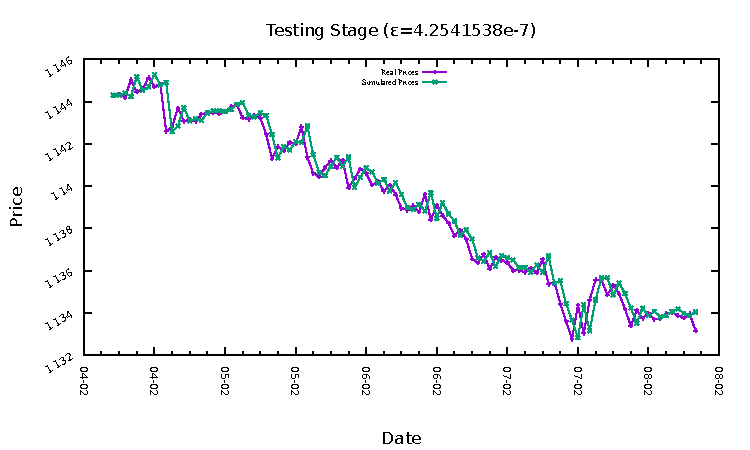
\includegraphics[width=.45\textwidth]{img/plots/eur_usd_h1-20agents-20rules-20ind-100gen_testing_fit.pdf}\quad
  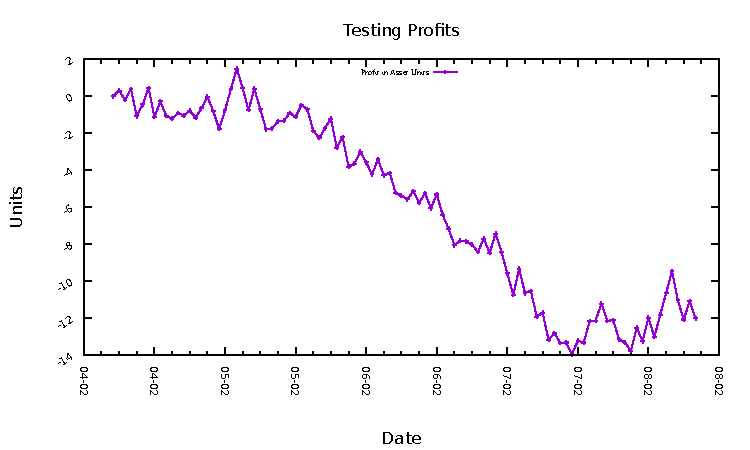
\includegraphics[width=.45\textwidth]{img/plots/eur_usd_h1-20agents-20rules-20ind-100gen_testing_profits.pdf}

  \medskip

  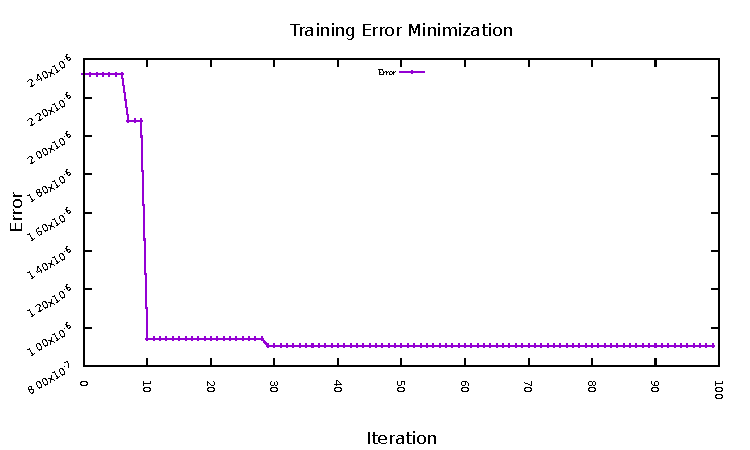
\includegraphics[width=.45\textwidth]{img/plots/eur_usd_h1-20agents-20rules-20ind-100gen_error_minimization.pdf}

  \caption{EUR/USD - 20 agents, 20 rules and 20 individuals}
  \label{pics:eur-usd-20agents-20rules-20individuals}
\end{figure}






\subsection{GBP/USD 4 Agents, 4 Rules, 4 Individuals}
\label{results:forecast-gbp-usd-4agents-4rules-4individuals}

\begin{figure}[htp]
  \centering

  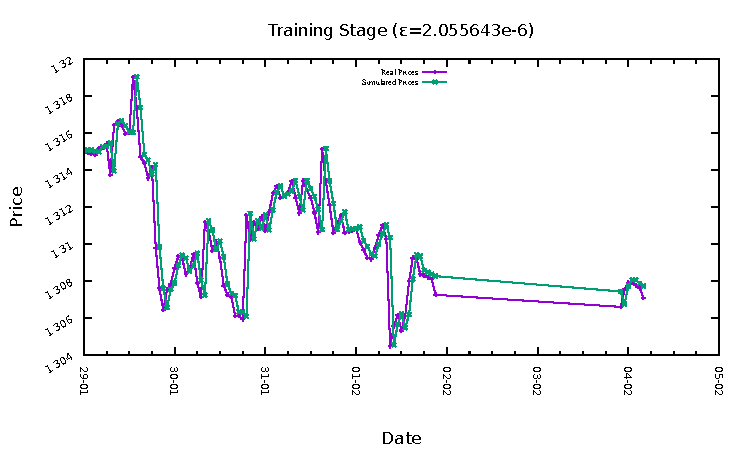
\includegraphics[width=.45\textwidth]{img/plots/gbp_usd_h1-4agents-4rules-4ind-100gen_training_fit.pdf}\quad
  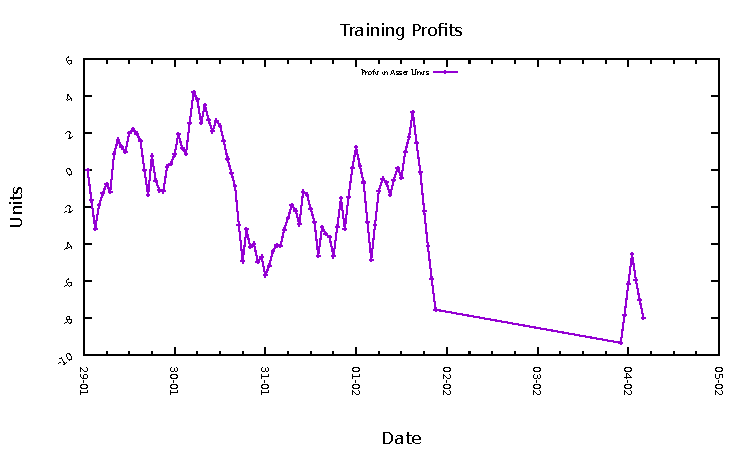
\includegraphics[width=.45\textwidth]{img/plots/gbp_usd_h1-4agents-4rules-4ind-100gen_training_profits.pdf}

  \medskip

  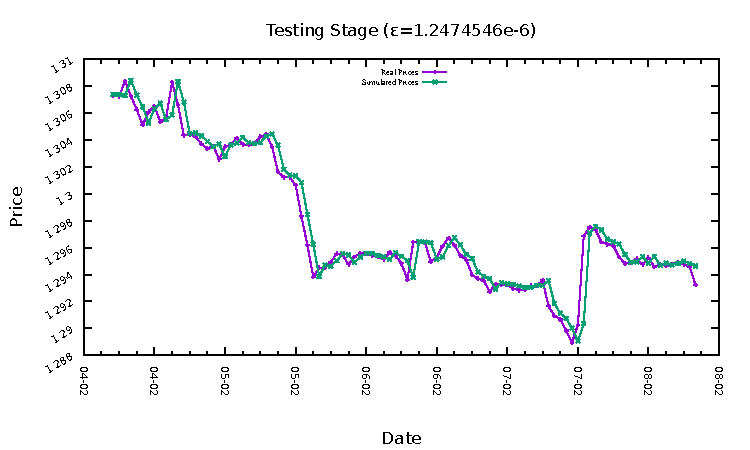
\includegraphics[width=.45\textwidth]{img/plots/gbp_usd_h1-4agents-4rules-4ind-100gen_testing_fit.pdf}\quad
  \includegraphics[width=.45\textwidth]{img/plots/gbp_usd_h1-4agents-4rules-4ind-100gen_testing_profits.pdf}

  \medskip

  \includegraphics[width=.45\textwidth]{img/plots/gbp_usd_h1-4agents-4rules-4ind-100gen_error_minimization.pdf}

  \caption{GBP/USD - 4 agents, 4 rules and 4 individuals}
  \label{pics:gbp-usd-4agents-4rules-4individuals}
\end{figure}

\subsection{GBP/USD 10 Agents, 10 Rules, 10 Individuals}
\label{results:forecast-gbp-usd-10agents-10rules-10individuals}

\begin{figure}[htp]
  \centering

  \includegraphics[width=.45\textwidth]{img/plots/gbp_usd_h1-10agents-10rules-10ind-100gen_training_fit.pdf}\quad
  \includegraphics[width=.45\textwidth]{img/plots/gbp_usd_h1-10agents-10rules-10ind-100gen_training_profits.pdf}

  \medskip

  \includegraphics[width=.45\textwidth]{img/plots/gbp_usd_h1-10agents-10rules-10ind-100gen_testing_fit.pdf}\quad
  \includegraphics[width=.45\textwidth]{img/plots/gbp_usd_h1-10agents-10rules-10ind-100gen_testing_profits.pdf}

  \medskip

  \includegraphics[width=.45\textwidth]{img/plots/gbp_usd_h1-10agents-10rules-10ind-100gen_error_minimization.pdf}

  \caption{GBP/USD - 10 agents, 10 rules and 10 individuals}
  \label{pics:gbp-usd-10agents-10rules-10individuals}
\end{figure}

\subsection{GBP/USD 20 Agents, 20 Rules, 20 Individuals}
\label{results:forecast-gbp-usd-20agents-20rules-20individuals}

\begin{figure}[htp]
  \centering

  \includegraphics[width=.45\textwidth]{img/plots/gbp_usd_h1-20agents-20rules-20ind-100gen_training_fit.pdf}\quad
  \includegraphics[width=.45\textwidth]{img/plots/gbp_usd_h1-20agents-20rules-20ind-100gen_training_profits.pdf}

  \medskip

  \includegraphics[width=.45\textwidth]{img/plots/gbp_usd_h1-20agents-20rules-20ind-100gen_testing_fit.pdf}\quad
  \includegraphics[width=.45\textwidth]{img/plots/gbp_usd_h1-20agents-20rules-20ind-100gen_testing_profits.pdf}

  \medskip

  \includegraphics[width=.45\textwidth]{img/plots/gbp_usd_h1-20agents-20rules-20ind-100gen_error_minimization.pdf}

  \caption{GBP/USD - 20 agents, 20 rules and 20 individuals}
  \label{pics:gbp-usd-20agents-20rules-20individuals}
\end{figure}









\subsection{USD/CAD 4 Agents, 4 Rules, 4 Individuals}
\label{results:forecast-usd-cad-4agents-4rules-4individuals}

\begin{figure}[htp]
  \centering

  \includegraphics[width=.45\textwidth]{img/plots/usd_cad_h1-4agents-4rules-4ind-100gen_training_fit.pdf}\quad
  \includegraphics[width=.45\textwidth]{img/plots/usd_cad_h1-4agents-4rules-4ind-100gen_training_profits.pdf}

  \medskip

  \includegraphics[width=.45\textwidth]{img/plots/usd_cad_h1-4agents-4rules-4ind-100gen_testing_fit.pdf}\quad
  \includegraphics[width=.45\textwidth]{img/plots/usd_cad_h1-4agents-4rules-4ind-100gen_testing_profits.pdf}

  \medskip

  \includegraphics[width=.45\textwidth]{img/plots/usd_cad_h1-4agents-4rules-4ind-100gen_error_minimization.pdf}

  \caption{USD/CAD - 4 agents, 4 rules and 4 individuals}
  \label{pics:usd-cad-4agents-4rules-4individuals}
\end{figure}

\subsection{USD/CAD 10 Agents, 10 Rules, 10 Individuals}
\label{results:forecast-usd-cad-10agents-10rules-10individuals}

\begin{figure}[htp]
  \centering

  \includegraphics[width=.45\textwidth]{img/plots/usd_cad_h1-10agents-10rules-10ind-100gen_training_fit.pdf}\quad
  \includegraphics[width=.45\textwidth]{img/plots/usd_cad_h1-10agents-10rules-10ind-100gen_training_profits.pdf}

  \medskip

  \includegraphics[width=.45\textwidth]{img/plots/usd_cad_h1-10agents-10rules-10ind-100gen_testing_fit.pdf}\quad
  \includegraphics[width=.45\textwidth]{img/plots/usd_cad_h1-10agents-10rules-10ind-100gen_testing_profits.pdf}

  \medskip

  \includegraphics[width=.45\textwidth]{img/plots/usd_cad_h1-10agents-10rules-10ind-100gen_error_minimization.pdf}

  \caption{USD/CAD - 10 agents, 10 rules and 10 individuals}
  \label{pics:usd-cad-10agents-10rules-10individuals}
\end{figure}

\subsection{USD/CAD 20 Agents, 20 Rules, 20 Individuals}
\label{results:forecast-usd-cad-20agents-20rules-20individuals}

\begin{figure}[htp]
  \centering

  \includegraphics[width=.45\textwidth]{img/plots/usd_cad_h1-20agents-20rules-20ind-100gen_training_fit.pdf}\quad
  \includegraphics[width=.45\textwidth]{img/plots/usd_cad_h1-20agents-20rules-20ind-100gen_training_profits.pdf}

  \medskip

  \includegraphics[width=.45\textwidth]{img/plots/usd_cad_h1-20agents-20rules-20ind-100gen_testing_fit.pdf}\quad
  \includegraphics[width=.45\textwidth]{img/plots/usd_cad_h1-20agents-20rules-20ind-100gen_testing_profits.pdf}

  \medskip

  \includegraphics[width=.45\textwidth]{img/plots/usd_cad_h1-20agents-20rules-20ind-100gen_error_minimization.pdf}

  \caption{USD/CAD - 20 agents, 20 rules and 20 individuals}
  \label{pics:usd-cad-20agents-20rules-20individuals}
\end{figure}




\section{Extracting Insights about a Financial Market}
\label{section:extracting-insights-about-a-financial-market}

\subsection{AUD/USD 4 Agents, 4 Rules, 4 Individuals}
\label{}

\subsubsection{Training}
\label{}

{\small
  \begin{itemize}
  \item 3 agents — with an average profit of -68 units — perceived in 68\% of
    the market that a weak resistance above current price — with a hesitancy of
    0.147 — is a signal to sell — with a hesitancy of 0.079.
  \item 2 agents — with an average profit of 280 units — perceived in 46\% of
    the market that a weak resistance nearby current price — with a hesitancy of
    0.133 — is a signal to buy — with a hesitancy of 0.097.
  \item 2 agents — with an average profit of 280 units — perceived in 22\% of
    the market that a moderate resistance above current price — with a hesitancy
    of 0.15 — is a signal to buy — with a hesitancy of 0.113.
  \item 2 agents — with an average profit of 38 units — perceived in 56\% of the
    market that a weak resistance below current price — with a hesitancy of
    0.246 — is a signal to buy — with a hesitancy of 0.094.
  \item 2 agents — with an average profit of -41 units — perceived in 56\% of
    the market that a weak resistance below current price — with a hesitancy of
    0.009 — is a signal to sell — with a hesitancy of 0.132.
  \end{itemize}
}

\subsubsection{Testing}
\label{}

{\small
  \begin{itemize}
  \item 3 agents — with an average profit of 68 units — perceived in 85\% of the
    market that a weak resistance above current price — with a hesitancy of
    0.147 — is a signal to sell — with a hesitancy of 0.079.
  \item 2 agents — with an average profit of 352 units — perceived in 47\% of
    the market that a moderate resistance below current price — with a hesitancy
    of 0.134 — is a signal to sell — with a hesitancy of 0.151.
  \item 2 agents — with an average profit of 323 units — perceived in 6\% of the
    market that a strong resistance below current price — with a hesitancy of
    0.098 — is a signal to sell — with a hesitancy of 0.024.
  \item 2 agents — with an average profit of 323 units — perceived in 55\% of
    the market that a weak resistance nearby current price — with a hesitancy of
    0.04 — is a signal to sell — with a hesitancy of 0.138.
  \item 2 agents — with an average profit of 309 units — perceived in 0\% of the
    market that a strong resistance above current price — with a hesitancy of
    0.127 — is a signal to sell — with a hesitancy of 0.14.
  \end{itemize}
}

\subsection{AUD/USD 10 Agents, 10 Rules, 10 Individuals}
\label{results:interpretation-aud-usd-10agents-10rules-10individuals}

\subsubsection{Training}

{\small
  \begin{itemize}
  \item 4 agents — with an average profit of 142 units — perceived in 32\% of the market that a moderate resistance above current price — with a hesitancy of 0.08 — is a signal to sell — with a hesitancy of 0.055.
  \item 4 agents — with an average profit of 115 units — perceived in 33\% of the market that a moderate resistance above current price — with a hesitancy of 0.111 — is a signal to buy — with a hesitancy of 0.044.
  \item 4 agents — with an average profit of 112 units — perceived in 28\% of the market that a moderate resistance above current price — with a hesitancy of 0.097 — is a signal to hold the current position — with a hesitancy of 0.128.
  \item 4 agents — with an average profit of 110 units — perceived in 34\% of the market that a moderate resistance below current price — with a hesitancy of 0.073 — is a signal to hold the current position — with a hesitancy of 0.241.
  \item 4 agents — with an average profit of 110 units — perceived in 63\% of the market that a weak resistance above current price — with a hesitancy of 0.128 — is a signal to hold the current position — with a hesitancy of 0.226.
  \end{itemize}
}

\subsubsection{Testing}

{\small
  \begin{itemize}
  \item 4 agents — with an average profit of -72 units — perceived in 1\% of the market that a strong resistance above current price — with a hesitancy of 0.122 — is a signal to buy — with a hesitancy of 0.098.
  \item 4 agents — with an average profit of -72 units — perceived in 41\% of the market that a moderate resistance nearby current price — with a hesitancy of 0.168 — is a signal to hold the current position — with a hesitancy of 0.41.
  \item 4 agents — with an average profit of -134 units — perceived in 55\% of the market that a moderate resistance below current price — with a hesitancy of 0.073 — is a signal to hold the current position — with a hesitancy of 0.241.
  \item 4 agents — with an average profit of -134 units — perceived in 85\% of the market that a weak resistance above current price — with a hesitancy of 0.128 — is a signal to hold the current position — with a hesitancy of 0.226.
  \item 4 agents — with an average profit of -134 units — perceived in 13\% of the market that a moderate resistance above current price — with a hesitancy of 0.097 — is a signal to hold the current position — with a hesitancy of 0.128.
  \end{itemize}
}

\subsection{AUD/USD 20 Agents, 20 Rules, 20 Individuals}
\label{}

\subsubsection{Training}
\label{}

{\small
  \begin{itemize}
  \item 4 agents — with an average profit of 201 units — perceived in 25\% of
    the market that a moderate resistance below current price — with a hesitancy
    of 0.22 — is a signal to buy — with a hesitancy of 0.068.
  \item 4 agents — with an average profit of 199 units — perceived in 20\% of
    the market that a strong resistance nearby current price — with a hesitancy
    of 0.088 — is a signal to buy — with a hesitancy of 0.107.
  \item 4 agents — with an average profit of 193 units — perceived in 26\% of
    the market that a moderate resistance above current price — with a hesitancy
    of 0.493 — is a signal to hold the current position — with a hesitancy of
    0.112.
  \item 4 agents — with an average profit of 183 units — perceived in 72\% of
    the market that a weak resistance above current price — with a hesitancy of
    0.114 — is a signal to buy — with a hesitancy of 0.096.
  \item 4 agents — with an average profit of 182 units — perceived in 11\% of
    the market that a strong resistance below current price — with a hesitancy
    of 0.092 — is a signal to buy — with a hesitancy of 0.104.
  \end{itemize}
}

\subsubsection{Testing}
\label{}

{\small
  \begin{itemize}
  \item 4 agents — with an average profit of -12 units — perceived in 13\% of
    the market that a strong resistance below current price — with a hesitancy
    of 0.163 — is a signal to sell — with a hesitancy of 0.058.
  \item 4 agents — with an average profit of -28 units — perceived in 49\% of
    the market that a weak resistance nearby current price — with a hesitancy of
    0.079 — is a signal to buy — with a hesitancy of 0.093.
  \item 4 agents — with an average profit of -77 units — perceived in 85\% of
    the market that a weak resistance above current price — with a hesitancy of
    0.06 — is a signal to hold the current position — with a hesitancy of 0.095.
  \item 4 agents — with an average profit of -77 units — perceived in 12\% of
    the market that a strong resistance nearby current price — with a hesitancy
    of 0.047 — is a signal to hold the current position — with a hesitancy of
    0.092.
  \item 4 agents — with an average profit of -77 units — perceived in 13\% of
    the market that a strong resistance below current price — with a hesitancy
    of 0.066 — is a signal to hold the current position — with a hesitancy of
    0.102.
  \end{itemize}
}



\subsection{EUR/GBP 4 Agents, 4 Rules, 4 Individuals}
\label{}

\subsubsection{Training}
\label{}

{\small
  \begin{itemize}
  \item 3 agents — with an average profit of 60 units — perceived in 56\% of
    the market that a weak resistance above current price — with a hesitancy
    of 0.094 — is a signal to hold the current position — with a hesitancy of
    0.029.
  \item 3 agents — with an average profit of 31 units — perceived in 36\% of the
    market that a moderate resistance nearby current price — with a hesitancy of
    0.126 — is a signal to hold the current position — with a hesitancy of 0.194.
  \item 3 agents — with an average profit of -44 units — perceived in 13\% of the
    market that a strong resistance below current price — with a hesitancy of
    0.044 — is a signal to hold the current position — with a hesitancy of 0.152.
  \item 2 agents — with an average profit of 105 units — perceived in 13\% of the
    market that a strong resistance below current price — with a hesitancy of
    0.114 — is a signal to sell — with a hesitancy of 0.102.
  \item 2 agents — with an average profit of 105 units — perceived in 42\% of the
    market that a weak resistance nearby current price — with a hesitancy of 0.105
    — is a signal to hold the current position — with a hesitancy of 0.048.
  \end{itemize}
}

\subsubsection{Testing}
\label{}

{\small
  \begin{itemize}
  \item 3 agents — with an average profit of 34 units — perceived in 79\% of
    the market that a weak resistance above current price — with a hesitancy
    of 0.094 — is a signal to hold the current position — with a hesitancy of
    0.029.
  \item 3 agents — with an average profit of 18 units — perceived in 33\% of the
    market that a moderate resistance nearby current price — with a hesitancy of
    0.126 — is a signal to hold the current position — with a hesitancy of 0.194.
  \item 3 agents — with an average profit of -23 units — perceived in 0\% of the
    market that a strong resistance below current price — with a hesitancy of
    0.044 — is a signal to hold the current position — with a hesitancy of 0.152.
  \item 2 agents — with an average profit of 60 units — perceived in 0\% of the
    market that a strong resistance below current price — with a hesitancy of
    0.114 — is a signal to sell — with a hesitancy of 0.102.
  \item 2 agents — with an average profit of 60 units — perceived in 57\% of the
    market that a weak resistance nearby current price — with a hesitancy of 0.105
    — is a signal to hold the current position — with a hesitancy of 0.048.
  \end{itemize}
}

\subsection{EUR/GBP 10 Agents, 10 Rules, 10 Individuals}
\label{results:interpretation-eur-gbp-10agents-10rules-10individuals}

\subsubsection{Training}

{\small
  \begin{itemize}
  \item 4 agents — with an average profit of -69 units — perceived in 22\% of the market that a moderate resistance below current price — with a hesitancy of 0.103 — is a signal to buy — with a hesitancy of 0.205.
  \item 4 agents — with an average profit of -70 units — perceived in 12\% of the market that a strong resistance below current price — with a hesitancy of 0.106 — is a signal to hold the current position — with a hesitancy of 0.108.
  \item 4 agents — with an average profit of -71 units — perceived in 12\% of the market that a strong resistance below current price — with a hesitancy of 0.103 — is a signal to sell — with a hesitancy of 0.053.
  \item 4 agents — with an average profit of -79 units — perceived in 38\% of the market that a moderate resistance above current price — with a hesitancy of 0.133 — is a signal to sell — with a hesitancy of 0.052.
  \item 4 agents — with an average profit of -100 units — perceived in 47\% of the market that a weak resistance nearby current price — with a hesitancy of 0.143 — is a signal to sell — with a hesitancy of 0.082.
  \end{itemize}
}

\subsubsection{Testing}

{\small
  \begin{itemize}
  \item 4 agents — with an average profit of -39 units — perceived in 27\% of the market that a moderate resistance below current price — with a hesitancy of 0.103 — is a signal to buy — with a hesitancy of 0.205.
  \item 4 agents — with an average profit of -40 units — perceived in 0\% of the market that a strong resistance below current price — with a hesitancy of 0.106 — is a signal to hold the current position — with a hesitancy of 0.108.
  \item 4 agents — with an average profit of -41 units — perceived in 0\% of the market that a strong resistance below current price — with a hesitancy of 0.103 — is a signal to sell — with a hesitancy of 0.053.
  \item 4 agents — with an average profit of -45 units — perceived in 18\% of the market that a moderate resistance above current price — with a hesitancy of 0.133 — is a signal to sell — with a hesitancy of 0.052.
  \item 4 agents — with an average profit of -57 units — perceived in 53\% of the market that a weak resistance nearby current price — with a hesitancy of 0.143 — is a signal to sell — with a hesitancy of 0.082.
  \end{itemize}
}

\subsection{EUR/GBP 20 Agents, 20 Rules, 20 Individuals}
\label{}

\subsubsection{Training}
\label{}

{\small
  \begin{itemize}
  \item 4 agents — with an average profit of 157 units — perceived in 42\% of
    the market that a moderate resistance above current price — with a
    hesitancy of 0.212 — is a signal to sell — with a hesitancy of 0.054.
  \item 4 agents — with an average profit of 146 units — perceived in 15\% of the
    market that a strong resistance nearby current price — with a hesitancy of
    0.28 — is a signal to hold the current position — with a hesitancy of 0.038.
  \item 4 agents — with an average profit of 144 units — perceived in 32\% of the
    market that a moderate resistance below current price — with a hesitancy of
    0.079 — is a signal to hold the current position — with a hesitancy of 0.07.
  \item 4 agents — with an average profit of 141 units — perceived in 56\% of the
    market that a weak resistance below current price — with a hesitancy of 0.066
    — is a signal to sell — with a hesitancy of 0.049.
  \item 4 agents — with an average profit of 135 units — perceived in 56\% of the
    market that a weak resistance below current price — with a hesitancy of 0.083
    — is a signal to hold the current position — with a hesitancy of 0.076.
  \end{itemize}
}

\subsubsection{Testing}
\label{}

{\small
  \begin{itemize}
  \item 4 agents — with an average profit of 85 units — perceived in 17\% of
    the market that a moderate resistance above current price — with a
    hesitancy of 0.212 — is a signal to sell — with a hesitancy of 0.054.
  \item 4 agents — with an average profit of 79 units — perceived in 7\% of the
    market that a strong resistance nearby current price — with a hesitancy of
    0.28 — is a signal to hold the current position — with a hesitancy of 0.038.
  \item 4 agents — with an average profit of 78 units — perceived in 30\% of the
    market that a moderate resistance below current price — with a hesitancy of
    0.079 — is a signal to hold the current position — with a hesitancy of 0.07.
  \item 4 agents — with an average profit of 76 units — perceived in 70\% of the
    market that a weak resistance below current price — with a hesitancy of 0.066
    — is a signal to sell — with a hesitancy of 0.049.
  \item 4 agents — with an average profit of 73 units — perceived in 70\% of the
    market that a weak resistance below current price — with a hesitancy of 0.083
    — is a signal to hold the current position — with a hesitancy of 0.076.
  \end{itemize}
}




\subsection{EUR/USD 4 Agents, 4 Rules, 4 Individuals}
\label{}

\subsubsection{Training}
\label{}

{\small
  \begin{itemize}
  \item 4 agents — with an average profit of 13 units — perceived in 21\% of the
    market that a moderate resistance above current price — with a hesitancy of
    0.072 — is a signal to hold the current position — with a hesitancy of
    0.089.
  \item 3 agents — with an average profit of 65 units — perceived in 33\% of the
    market that a moderate resistance nearby current price — with a hesitancy of
    0.037 — is a signal to sell — with a hesitancy of 0.279.
  \item 3 agents — with an average profit of 53 units — perceived in 21\% of the
    market that a moderate resistance above current price — with a hesitancy of
    0.155 — is a signal to sell — with a hesitancy of 0.093.
  \item 3 agents — with an average profit of 52 units — perceived in 66\% of the
    market that a weak resistance below current price — with a hesitancy of
    0.124 — is a signal to sell — with a hesitancy of 0.23.
  \item 3 agents — with an average profit of 29 units — perceived in 31\% of the
    market that a moderate resistance nearby current price — with a hesitancy of
    0.092 — is a signal to hold the current position — with a hesitancy of
    0.075.
  \end{itemize}
}

\subsubsection{Testing}
\label{}

{\small
  \begin{itemize}
  \item 4 agents — with an average profit of 14 units — perceived in 16\% of
    the market that a moderate resistance above current price — with a
    hesitancy of 0.072 — is a signal to hold the current position — with a
    hesitancy of 0.089.
  \item 3 agents — with an average profit of 19 units — perceived in 46\% of the
    market that a moderate resistance nearby current price — with a hesitancy of
    0.092 — is a signal to hold the current position — with a hesitancy of 0.075.
  \item 3 agents — with an average profit of -3 units — perceived in 20\% of the
    market that a weak resistance below current price — with a hesitancy of 0.124
    — is a signal to sell — with a hesitancy of 0.23.
  \item 3 agents — with an average profit of -7 units — perceived in 15\% of the
    market that a moderate resistance above current price — with a hesitancy of
    0.155 — is a signal to sell — with a hesitancy of 0.093.
  \item 3 agents — with an average profit of -22 units — perceived in 23\% of the
    market that a weak resistance below current price — with a hesitancy of 0.063
    — is a signal to hold the current position — with a hesitancy of 0.092.
  \end{itemize}
}

\subsection{EUR/USD 10 Agents, 10 Rules, 10 Individuals}
\label{results:interpretation-eur-usd-10agents-10rules-10individuals}

\subsubsection{Training}

{\small
  \begin{itemize}
  \item 4 agents — with an average profit of 0 units — perceived in 76\% of the market that a weak resistance below current price — with a hesitancy of 0.051 — is a signal to hold the current position — with a hesitancy of 0.056.
  \item 4 agents — with an average profit of -20 units — perceived in 9\% of the market that a strong resistance below current price — with a hesitancy of 0.109 — is a signal to buy — with a hesitancy of 0.055.
  \item 4 agents — with an average profit of -24 units — perceived in 46\% of the market that a weak resistance nearby current price — with a hesitancy of 0.115 — is a signal to buy — with a hesitancy of 0.044.
  \item 4 agents — with an average profit of -24 units — perceived in 27\% of the market that a strong resistance nearby current price — with a hesitancy of 0.097 — is a signal to sell — with a hesitancy of 0.038.
  \item 4 agents — with an average profit of -44 units — perceived in 47\% of the market that a weak resistance nearby current price — with a hesitancy of 0.226 — is a signal to hold the current position — with a hesitancy of 0.13.
  \end{itemize}
}

\subsubsection{Testing}

{\small
  \begin{itemize}
  \item 4 agents — with an average profit of -3 units — perceived in 30\% of the market that a weak resistance below current price — with a hesitancy of 0.051 — is a signal to hold the current position — with a hesitancy of 0.056.
  \item 4 agents — with an average profit of -64 units — perceived in 9\% of the market that a strong resistance below current price — with a hesitancy of 0.109 — is a signal to buy — with a hesitancy of 0.055.
  \item 4 agents — with an average profit of -79 units — perceived in 41\% of the market that a weak resistance nearby current price — with a hesitancy of 0.115 — is a signal to buy — with a hesitancy of 0.044.
  \item 4 agents — with an average profit of -79 units — perceived in 11\% of the market that a strong resistance nearby current price — with a hesitancy of 0.097 — is a signal to sell — with a hesitancy of 0.038.
  \item 4 agents — with an average profit of -138 units — perceived in 42\% of the market that a weak resistance nearby current price — with a hesitancy of 0.226 — is a signal to hold the current position — with a hesitancy of 0.13.
  \end{itemize}
}

\subsection{EUR/USD 20 Agents, 20 Rules, 20 Individuals}
\label{}

\subsubsection{Training}
\label{}

{\small
  \begin{itemize}
  \item 4 agents — with an average profit of -10 units — perceived in 21\% of
    the market that a strong resistance nearby current price — with a
    hesitancy of 0.347 — is a signal to sell — with a hesitancy of 0.067.
  \item 4 agents — with an average profit of -12 units — perceived in 18\% of the
    market that a moderate resistance below current price — with a hesitancy of
    0.156 — is a signal to sell — with a hesitancy of 0.1.
  \item 4 agents — with an average profit of -12 units — perceived in 72\% of the
    market that a weak resistance above current price — with a hesitancy of 0.077
    — is a signal to buy — with a hesitancy of 0.217.
  \item 4 agents — with an average profit of -22 units — perceived in 46\% of the
    market that a weak resistance nearby current price — with a hesitancy of 0.065
    — is a signal to buy — with a hesitancy of 0.097.
  \item 4 agents — with an average profit of -29 units — perceived in 4\% of the
    market that a strong resistance above current price — with a hesitancy of
    0.103 — is a signal to sell — with a hesitancy of 0.068.
  \end{itemize}
}

\subsubsection{Testing}
\label{}

{\small
  \begin{itemize}
  \item 4 agents — with an average profit of -30 units — perceived in 11\% of
    the market that a strong resistance nearby current price — with a
    hesitancy of 0.347 — is a signal to sell — with a hesitancy of 0.067.
  \item 4 agents — with an average profit of -35 units — perceived in 57\% of the
    market that a moderate resistance below current price — with a hesitancy of
    0.156 — is a signal to sell — with a hesitancy of 0.1.
  \item 4 agents — with an average profit of -35 units — perceived in 93\% of the
    market that a weak resistance above current price — with a hesitancy of 0.077
    — is a signal to buy — with a hesitancy of 0.217.
  \item 4 agents — with an average profit of -67 units — perceived in 44\% of the
    market that a weak resistance nearby current price — with a hesitancy of 0.065
    — is a signal to buy — with a hesitancy of 0.097.
  \item 4 agents — with an average profit of -87 units — perceived in 0\% of the
    market that a strong resistance above current price — with a hesitancy of
    0.103 — is a signal to sell — with a hesitancy of 0.068.
  \end{itemize}
}





\subsection{GBP/USD 4 Agents, 4 Rules, 4 Individuals}
\label{}

\subsubsection{Training}
\label{}

{\small
  \begin{itemize}
  \item 3 agents — with an average profit of 88 units — perceived in 37\% of
    the market that a weak resistance nearby current price — with a hesitancy
    of 0.055 — is a signal to hold the current position — with a hesitancy of
    0.105.
  \item 3 agents — with an average profit of -92 units — perceived in 29\% of the
    market that a moderate resistance above current price — with a hesitancy of
    0.139 — is a signal to hold the current position — with a hesitancy of 0.085.
  \item 3 agents — with an average profit of -155 units — perceived in 10\% of the
    market that a strong resistance above current price — with a hesitancy of
    0.018 — is a signal to buy — with a hesitancy of 0.112.
  \item 3 agents — with an average profit of -156 units — perceived in 46\% of the
    market that a moderate resistance nearby current price — with a hesitancy of
    0.107 — is a signal to buy — with a hesitancy of 0.125.
  \item 3 agents — with an average profit of -156 units — perceived in 46\% of the
    market that a moderate resistance nearby current price — with a hesitancy of
    0.137 — is a signal to hold the current position — with a hesitancy of 0.108.
  \end{itemize}
}

\subsubsection{Testing}
\label{}

{\small
  \begin{itemize}
  \item 3 agents — with an average profit of 169 units — perceived in 46\% of
    the market that a weak resistance nearby current price — with a hesitancy
    of 0.055 — is a signal to hold the current position — with a hesitancy of
    0.105.
  \item 3 agents — with an average profit of -178 units — perceived in 13\% of the
    market that a moderate resistance above current price — with a hesitancy of
    0.139 — is a signal to hold the current position — with a hesitancy of 0.085.
  \item 3 agents — with an average profit of -300 units — perceived in 10\% of the
    market that a strong resistance above current price — with a hesitancy of
    0.018 — is a signal to buy — with a hesitancy of 0.112.
  \item 3 agents — with an average profit of -302 units — perceived in 32\% of the
    market that a moderate resistance nearby current price — with a hesitancy of
    0.107 — is a signal to buy — with a hesitancy of 0.125.
  \item 3 agents — with an average profit of -302 units — perceived in 32\% of the
    market that a moderate resistance nearby current price — with a hesitancy of
    0.137 — is a signal to hold the current position — with a hesitancy of 0.108.
  \end{itemize}
}

\subsection{GBP/USD 10 Agents, 10 Rules, 10 Individuals}
\label{results:interpretation-gbp-usd-10agents-10rules-10individuals}

\subsubsection{Training}

{\small
  \begin{itemize}
  \item 4 agents — with an average profit of 52 units — perceived in 18\% of the market that a strong resistance nearby current price — with a hesitancy of 0.047 — is a signal to buy — with a hesitancy of 0.138.
  \item 4 agents — with an average profit of 48 units — perceived in 32\% of the market that a moderate resistance above current price — with a hesitancy of 0.155 — is a signal to hold the current position — with a hesitancy of 0.084.
  \item 4 agents — with an average profit of 48 units — perceived in 42\% of the market that a moderate resistance below current price — with a hesitancy of 0.098 — is a signal to hold the current position — with a hesitancy of 0.133.
  \item 4 agents — with an average profit of 39 units — perceived in 32\% of the market that a moderate resistance above current price — with a hesitancy of 0.154 — is a signal to buy — with a hesitancy of 0.085.
  \item 4 agents — with an average profit of 37 units — perceived in 59\% of the market that a weak resistance above current price — with a hesitancy of 0.124 — is a signal to sell — with a hesitancy of 0.118.
  \end{itemize}
}

\subsubsection{Testing}

{\small
  \begin{itemize}
  \item 4 agents — with an average profit of 96 units — perceived in 24\% of the market that a strong resistance nearby current price — with a hesitancy of 0.047 — is a signal to buy — with a hesitancy of 0.138.
  \item 4 agents — with an average profit of 88 units — perceived in 44\% of the market that a moderate resistance below current price — with a hesitancy of 0.098 — is a signal to hold the current position — with a hesitancy of 0.133.
  \item 4 agents — with an average profit of 87 units — perceived in 16\% of the market that a moderate resistance above current price — with a hesitancy of 0.155 — is a signal to hold the current position — with a hesitancy of 0.084.
  \item 4 agents — with an average profit of 62 units — perceived in 16\% of the market that a moderate resistance above current price — with a hesitancy of 0.154 — is a signal to buy — with a hesitancy of 0.085.
  \item 4 agents — with an average profit of 58 units — perceived in 35\% of the market that a moderate resistance nearby current price — with a hesitancy of 0.194 — is a signal to sell — with a hesitancy of 0.511.
  \end{itemize}
}

\subsection{GBP/USD 20 Agents, 20 Rules, 20 Individuals}
\label{}

\subsubsection{Training}
\label{}

{\small
  \begin{itemize}
  \item 4 agents — with an average profit of -118 units — perceived in 56\% of
    the market that a weak resistance above current price — with a hesitancy
    of 0.054 — is a signal to hold the current position — with a hesitancy of
    0.104.
  \item 4 agents — with an average profit of -118 units — perceived in 44\% of the
    market that a weak resistance nearby current price — with a hesitancy of 0.087
    — is a signal to buy — with a hesitancy of 0.044.
  \item 4 agents — with an average profit of -160 units — perceived in 32\% of the
    market that a moderate resistance above current price — with a hesitancy of
    0.175 — is a signal to hold the current position — with a hesitancy of 0.111.
  \item 4 agents — with an average profit of -176 units — perceived in 57\% of the
    market that a weak resistance above current price — with a hesitancy of 0.105
    — is a signal to sell — with a hesitancy of 0.158.
  \item 4 agents — with an average profit of -190 units — perceived in 32\% of the
    market that a moderate resistance above current price — with a hesitancy of
    0.233 — is a signal to buy — with a hesitancy of 0.074.
  \end{itemize}
}

\subsubsection{Testing}
\label{}

{\small
  \begin{itemize}
  \item 4 agents — with an average profit of -227 units — perceived in 67\% of
    the market that a weak resistance above current price — with a hesitancy
    of 0.054 — is a signal to hold the current position — with a hesitancy of
    0.104.
  \item 4 agents — with an average profit of -227 units — perceived in 41\% of the
    market that a weak resistance nearby current price — with a hesitancy of 0.087
    — is a signal to buy — with a hesitancy of 0.044.
  \item 4 agents — with an average profit of -309 units — perceived in 27\% of the
    market that a moderate resistance above current price — with a hesitancy of
    0.175 — is a signal to hold the current position — with a hesitancy of 0.111.
  \item 4 agents — with an average profit of -341 units — perceived in 63\% of the
    market that a weak resistance above current price — with a hesitancy of 0.105
    — is a signal to sell — with a hesitancy of 0.158.
  \item 4 agents — with an average profit of -368 units — perceived in 28\% of the
    market that a moderate resistance above current price — with a hesitancy of
    0.233 — is a signal to buy — with a hesitancy of 0.074.
  \end{itemize}
}





\subsection{USD/CAD 4 Agents, 4 Rules, 4 Individuals}
\label{}

\subsubsection{Training}
\label{}

{\small
  \begin{itemize}
  \item 4 agents — with an average profit of 25 units — perceived in 6\% of
    the market that a strong resistance above current price — with a hesitancy
    of 0.157 — is a signal to buy — with a hesitancy of 0.104.
  \item 3 agents — with an average profit of 48 units — perceived in 41\% of the
    market that a weak resistance nearby current price — with a hesitancy of 0.041
    — is a signal to hold the current position — with a hesitancy of 0.238.
  \item 3 agents — with an average profit of 37 units — perceived in 60\% of the
    market that a weak resistance above current price — with a hesitancy of 0.093
    — is a signal to hold the current position — with a hesitancy of 0.239.
  \item 3 agents — with an average profit of 37 units — perceived in 60\% of the
    market that a weak resistance above current price — with a hesitancy of 0.071
    — is a signal to sell — with a hesitancy of 0.072.
  \item 3 agents — with an average profit of 14 units — perceived in 36\% of the
    market that a moderate resistance below current price — with a hesitancy of
    0.451 — is a signal to sell — with a hesitancy of 0.062.
  \end{itemize}
}

\subsubsection{Testing}
\label{}

{\small
  \begin{itemize}
  \item 4 agents — with an average profit of -44 units — perceived in 17\% of
    the market that a strong resistance above current price — with a hesitancy
    of 0.157 — is a signal to buy — with a hesitancy of 0.104.
  \item 3 agents — with an average profit of 59 units — perceived in 18\% of the
    market that a moderate resistance below current price — with a hesitancy of
    0.106 — is a signal to hold the current position — with a hesitancy of 0.045.
  \item 3 agents — with an average profit of -23 units — perceived in 19\% of the
    market that a moderate resistance below current price — with a hesitancy of
    0.451 — is a signal to sell — with a hesitancy of 0.062.
  \item 3 agents — with an average profit of -64 units — perceived in 47\% of the
    market that a weak resistance above current price — with a hesitancy of 0.093
    — is a signal to hold the current position — with a hesitancy of 0.239.
  \item 3 agents — with an average profit of -64 units — perceived in 47\% of the
    market that a weak resistance above current price — with a hesitancy of 0.071
    — is a signal to sell — with a hesitancy of 0.072.
  \end{itemize}
}

\subsection{USD/CAD 10 Agents, 10 Rules, 10 Individuals}
\label{results:interpretation-usd-cad-10agents-10rules-10individuals}

\subsubsection{Training}

{\small
  \begin{itemize}
  \item 9 agents — with an average profit of 343 units — perceived in 49\% of the market that a moderate resistance nearby current price — with a hesitancy of 0.097 — is a signal to sell — with a hesitancy of 0.115.
  \item 9 agents — with an average profit of 273 units — perceived in 16\% of the market that a strong resistance nearby current price — with a hesitancy of 0.173 — is a signal to sell — with a hesitancy of 0.087.
  \item 8 agents — with an average profit of 439 units — perceived in 39\% of the market that a moderate resistance above current price — with a hesitancy of 0.131 — is a signal to sell — with a hesitancy of 0.24.
  \item 8 agents — with an average profit of 425 units — perceived in 7\% of the market that a strong resistance above current price — with a hesitancy of 0.081 — is a signal to buy — with a hesitancy of 0.028.
  \item 8 agents — with an average profit of 401 units — perceived in 53\% of the market that a weak resistance below current price — with a hesitancy of 0.233 — is a signal to hold the current position — with a hesitancy of 0.124.
  \end{itemize}
}

\subsubsection{Testing}

{\small
  \begin{itemize}
  \item 9 agents — with an average profit of -483 units — perceived in 22\% of the market that a strong resistance nearby current price — with a hesitancy of 0.173 — is a signal to sell — with a hesitancy of 0.087.
  \item 9 agents — with an average profit of -607 units — perceived in 40\% of the market that a moderate resistance nearby current price — with a hesitancy of 0.097 — is a signal to sell — with a hesitancy of 0.115.
  \item 8 agents — with an average profit of -441 units — perceived in 74\% of the market that a weak resistance below current price — with a hesitancy of 0.101 — is a signal to sell — with a hesitancy of 0.091.
  \item 8 agents — with an average profit of -442 units — perceived in 45\% of the market that a weak resistance above current price — with a hesitancy of 0.083 — is a signal to sell — with a hesitancy of 0.073.
  \item 8 agents — with an average profit of -602 units — perceived in 44\% of the market that a weak resistance above current price — with a hesitancy of 0.123 — is a signal to hold the current position — with a hesitancy of 0.131.
  \end{itemize}
}

\subsection{USD/CAD 20 Agents, 20 Rules, 20 Individuals}
\label{}

\subsubsection{Training}
\label{}

{\small
  \begin{itemize}
  \item 4 agents — with an average profit of -106 units — perceived in 56\% of
    the market that a weak resistance above current price — with a hesitancy
    of 0.06 — is a signal to sell — with a hesitancy of 0.203.
  \item 4 agents — with an average profit of -106 units — perceived in 37\% of the
    market that a moderate resistance below current price — with a hesitancy of
    0.077 — is a signal to sell — with a hesitancy of 0.125.
  \item 4 agents — with an average profit of -142 units — perceived in 38\% of the
    market that a moderate resistance below current price — with a hesitancy of
    0.052 — is a signal to buy — with a hesitancy of 0.092.
  \item 4 agents — with an average profit of -160 units — perceived in 50\% of the
    market that a weak resistance below current price — with a hesitancy of 0.049
    — is a signal to sell — with a hesitancy of 0.079.
  \item 4 agents — with an average profit of -169 units — perceived in 11\% of the
    market that a strong resistance below current price — with a hesitancy of
    0.178 — is a signal to sell — with a hesitancy of 0.194.
  \end{itemize}
}

\subsubsection{Testing}
\label{}

{\small
  \begin{itemize}
  \item 4 agents — with an average profit of 433 units — perceived in 10\% of
    the market that a strong resistance below current price — with a hesitancy
    of 0.066 — is a signal to buy — with a hesitancy of 0.073.
  \item 4 agents — with an average profit of 432 units — perceived in 18\% of the
    market that a strong resistance nearby current price — with a hesitancy of
    0.075 — is a signal to hold the current position — with a hesitancy of 0.059.
  \item 4 agents — with an average profit of 420 units — perceived in 10\% of the
    market that a strong resistance below current price — with a hesitancy of
    0.083 — is a signal to hold the current position — with a hesitancy of 0.103.
  \item 4 agents — with an average profit of 413 units — perceived in 38\% of the
    market that a moderate resistance nearby current price — with a hesitancy of
    0.124 — is a signal to hold the current position — with a hesitancy of 0.072.
  \item 4 agents — with an average profit of 412 units — perceived in 40\% of the
    market that a moderate resistance above current price — with a hesitancy of
    0.063 — is a signal to buy — with a hesitancy of 0.115.
  \end{itemize}
}
